
\section{二叉查找树}

在一组混乱、无序的线性表中查找关键字为某值的数据，平均时间复杂度为O(n)。若数据存放在有序的顺序表中，使用二分查找平均时间复杂度可以达到O(logn)。但是顺序表难以维护动态数据：
当表中元素增加或删除时，需要移动大量元素，移动操作的平均时间复杂度为O(n)。

二叉查找树的思想类似二分查找，将元素通过某种有序的方式组织起来，以达到较为高效的元素查找效率。经过本节的研究我们将看到，
在二叉查找树中查找元素的\uline{平均}时间复杂度为O(logn)，插入、删除元素的\uline{平均}时间复杂度同样是O(logn)。

\begin{definitionbox}
    \term{二叉查找树}要么是一棵空树，要么是：\\

    一棵由根节点、左子树和右子树构成的二叉树，其中左子树和右子树均是二叉查找树，并且左子树上所有节点的关键字均小于根节点的关键字，右子树上所有节点的
    关键字均大于根节点的关键字。
\end{definitionbox}
图\ref{fig:几棵不同的二叉查找树}展示了几棵不同的二叉查找树。
\begin{figure}[htbp]
    \centering
    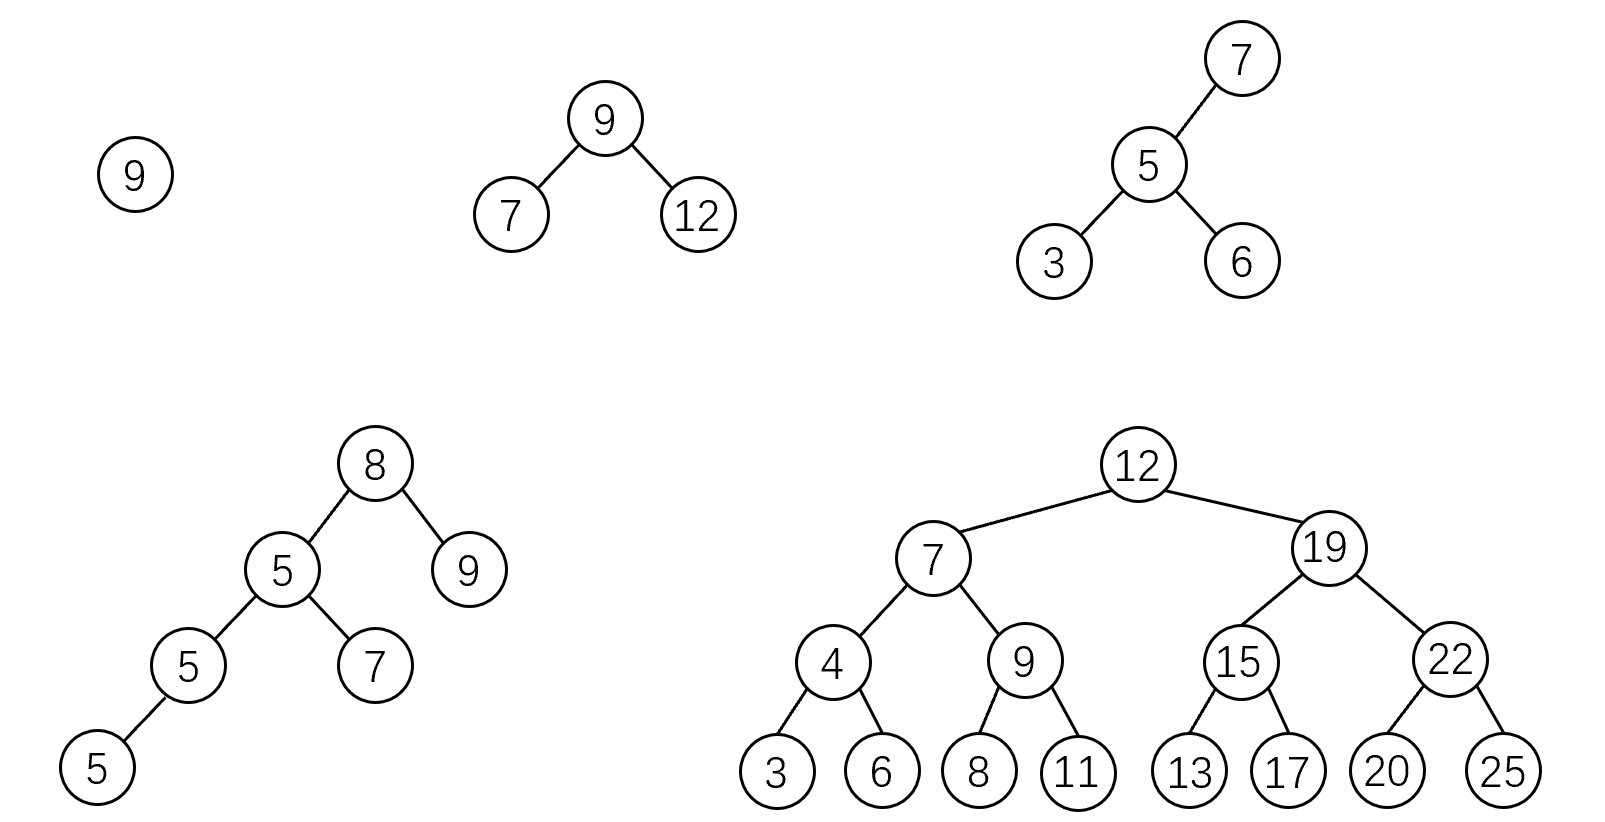
\includegraphics[width=0.78\textwidth]{assets/pics_and_ppts/ch4/几棵不同的二叉查找树.png}
    \caption{几棵不同的二叉查找树}
    \label{fig:几棵不同的二叉查找树}
\end{figure}
可以看到，二叉查找树其实是一种\uline{有序}的树形结构。二叉查找树具有“左小、根中、右大”的特征，而按照中序遍历“左-根-右”的方式遍历二叉查找树，得到
的序列就是一个有序序列。

二叉查找树最重要的意义就在于在动态变化的数据中较为高效地进行查找，如前文所述，其查找、插入和删除均能达到O(logn)的平均时间复杂度。接下来我们就来看看如何实现这些操作。

\subsection{二叉查找树的实现}
通常情况下，二叉查找树同样采用二叉链表实现：
\begin{cppcode}
    struct BSTreeNode { // Binary Search Tree
        ElemType data;  
        BSTreeNode* lchild;
        BSTreeNode* rchild;
    };
\end{cppcode}
为不引入额外的理解负担，我们假设data已经是某种可以比较大小的数据结构，data本身即作为关键字。

\minisection{1.查找操作}
如何在二叉查找树T中，查找关键字值为e的元素？

由于二叉查找树的特点，根节点其实作为分界线，将左右两棵子树划分成了“两个界域”，若e的值大于根节点，则它不可能出现在左子树中，如图\ref{fig:根节点划分界域}，
直接递归地在右子树中查找即可。
\begin{figure}[htbp]
    \centering
    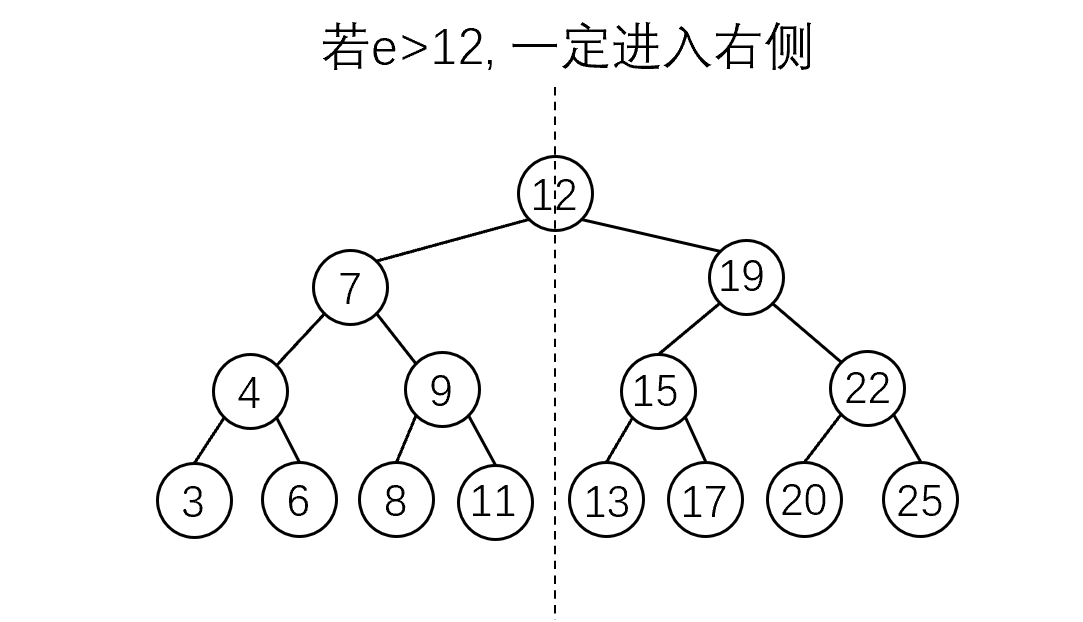
\includegraphics[width=0.58\textwidth]{assets/pics_and_ppts/ch4/根节点划分界域.png}
    \caption{}
    \label{fig:根节点划分界域}
    
\end{figure}

类似地，若e更小，则它不可能出现在左子树中。因此在二叉查找树中查找元素，不必像无序线性表那样将所有元素遍历一遍，而是可以舍弃掉大量元素的比较，因此效率更高。
如果e存在，一定会在查找过程中找到。如果e不存在，则递归一定会进行到某个空节点。


具体来说，查找过程如下：从根节点开始，
\begin{enumerate}
    \item 若当前节点为空，说明查找失败，返回；否则进入第2步。
    \item 若e的值等于当前节点，说明查找成功，访问它；
    \item 若e的值小于当前节点，说明应该往左，因此递归地在当前节点的左子树中查找；
    \item 若e的值大于当前节点，说明应该往右，因此递归地在当前节点的右子树中查找。
\end{enumerate}
代码如下所示：

\begin{cppcode}
    int BSTSearch(BSTreeNode* root, ElemType e) {
        if(root == NULL) {
            return 0;   // 查找失败，e不存在
        }
        if(e == root->data) {
            visit(root);    // 找到了，做你想对它做的事吧！
            return 1;   // 查找成功
        }
        if(e > root->data) {
            return BSTSearch(root->rchild, e);
        }
        if(e < root->data) {
            return BSTSearch(root->lchild, e);
        }

    }
\end{cppcode}
在图\ref{fig:二叉查找树的查找过程}所示的二叉树中查找8和查找21的过程如图所示。

\begin{figure}
    \centering
    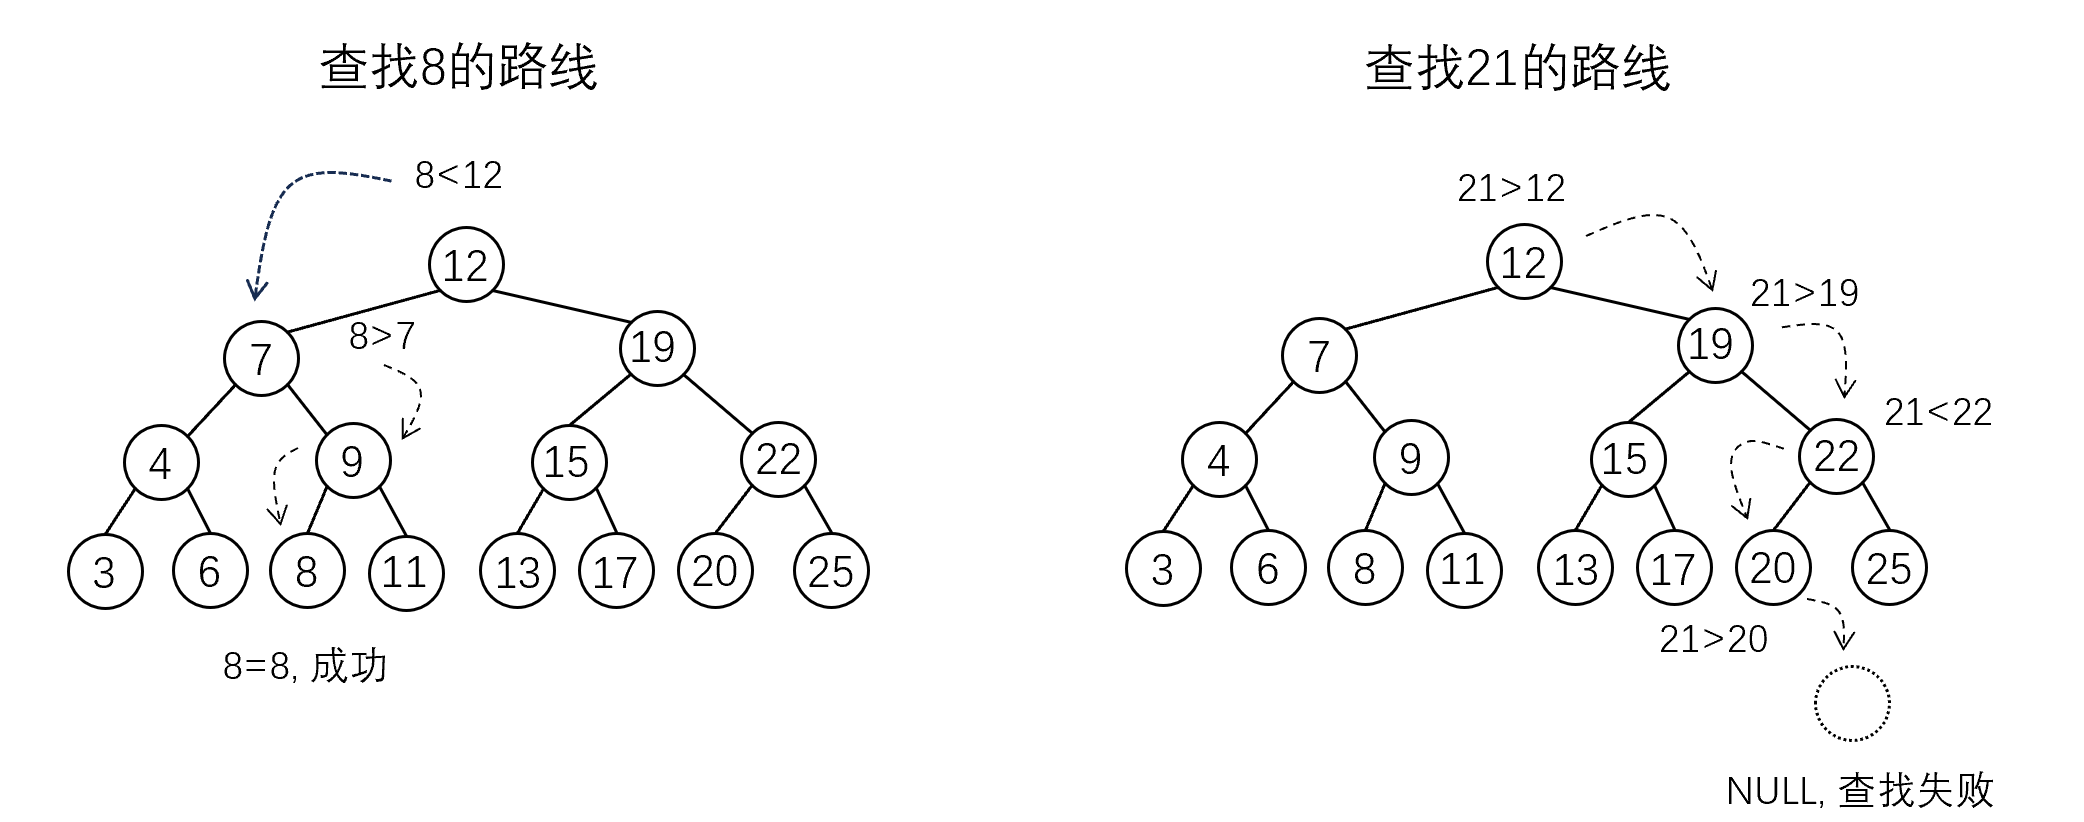
\includegraphics[width=0.88\textwidth]{assets/pics_and_ppts/ch4/二叉查找树的查找过程.png}
    \caption{}
    \label{fig:二叉查找树的查找过程}
\end{figure}
显然\uline{平均情况下}，若二叉树中有n个节点，比较次数约为log(n) / 2，因此查找的平均时间复杂度为O(logn)。


\minisection{2.插入操作}
插入节点时，可以从根节点开始，将根节点元素与待插元素比较。若待插元素较小，则说明该节点需要在左子树中插入，此时，若：\\
\Circled{1} 左子树为空，则插入位置已经找到，直接插入；\\
\Circled{2} 左子树非空，则递归地进入左子树，进行同样的操作。\\
反之若待插元素大于根节点，则递归地进入右子树。如此递归进行下去，直至找到正确的位置。具体实现代码如下：

\begin{cppcode}
    void InsertBSTree(node* &root, int e) {
        if(root == NULL) {
            // 空树，直接插入就行
            node* new_node = (node*)malloc(sizeof(node));
            new_node->data = e;
            new_node->lchild = NULL;
            new_node->rchild = NULL;
            root = new_node;
            return ;
        }
        // e已存在，无需插入
        if(e == root->data) {
            return ;
        }
        if(e < root->data) {   // 待插元素较小
            // 递归地进入左子树
            InsertBSTree(root->lchild, e);    
        } 
        else if(e > root->data) {    // 待插元素较大
            // 递归地进入右子树
            InsertBSTree(root->rchild, e);    
        }
    }
\end{cppcode}
在图\ref{fig:二叉查找树的插入过程}所示的二叉树中分别插入8和插入21的过程如图所示。注意上面的代码中，root变量作为根节点的地址，该地址本身是有可能
被修改的，因此一定要以引用作为参数，而不能是普通的拷贝传递。
\begin{figure}
    \centering
    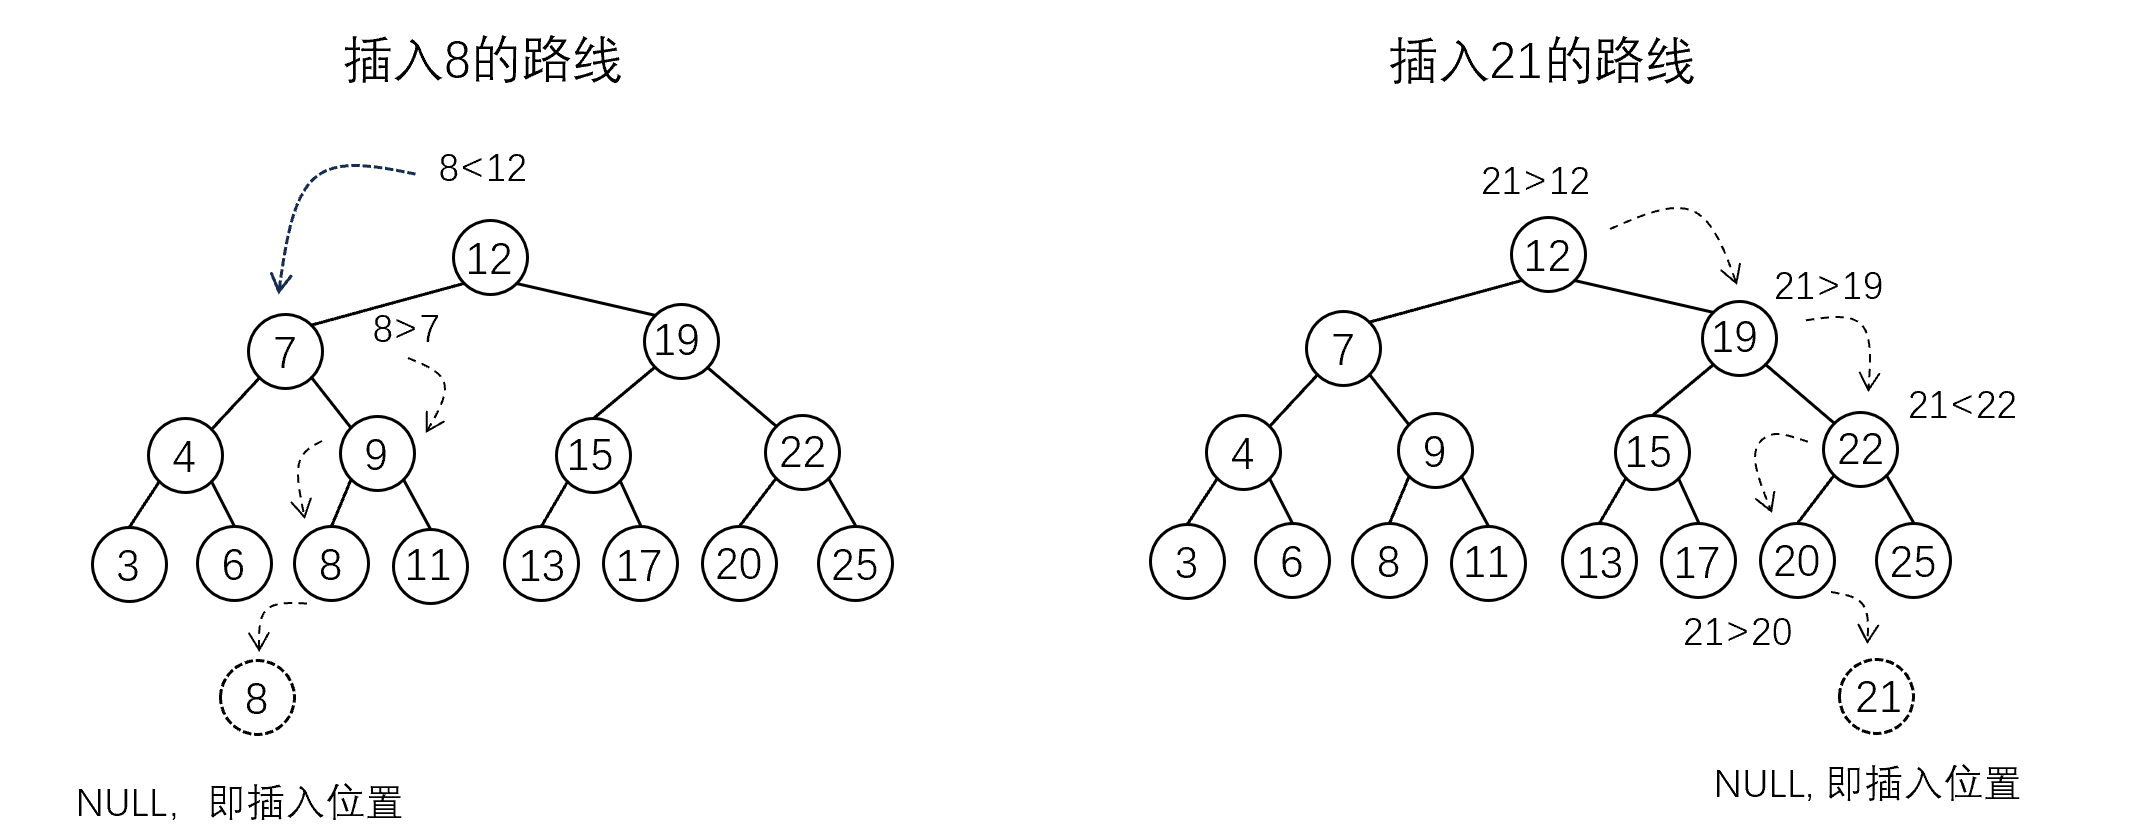
\includegraphics[width=0.89\textwidth]{assets/pics_and_ppts/ch4/二叉查找树的插入过程.png}
    \caption{}
    \label{fig:二叉查找树的插入过程}
\end{figure}

\minisection{3.由已有数据建立二叉查找树}
假设数组arr[]中存放了n个数据，用这些数据建立一棵二叉查找树的过程，其实就是将它们一一插入二叉查找树的过程。代码如下所示：
\begin{cppcode}
    BSTreeNode* CreateBSTree(ElemType arr[], int n) {
        BSTreeNode* root = NULL;
        for(int i=0; i<n; i++) {
            InsertBSTree(root, arr[i]);
        }
        return root;
    }
\end{cppcode}
需要注意的是，即使是同样的一组数据，如果插入它们的顺序不同，也可能生成不同的二叉查找树。例如插入顺序为{1,2,3,4,5,6,7,8,9}，会得到一棵“斜向右下的一条直线”的树，深度
为9；而插入顺序为{9,8,7,6,5,4,3,2,1}，树形则会是“斜向左下的一条直线”。


\minisection{4.删除操作}
在二叉查找树T中删除关键字为e的节点，如何做？

与插入操作不同，插入操作一定能“陷入”一棵空树作为插入位置，而对于删除操作，被删节点很可能还有复杂的子树。显然：

\Circled{1} 对于待删节点是叶节点，直接释放掉该节点即可。

\Circled{2} 若待删节点是非叶节点，该怎么办呢？常见的做法是找到待删节点的\term{中序前驱}或\term{中序后继}，用中序前驱或中序后继覆盖掉待删节点，
然后问题便转化成了递归地在左子树中删除中序前驱，或在右子树中删除中序后继，如此向子树递归、向子树的子树递归、向子树的子树的子树递归......
总会将问题\uwave{化归}为\Circled{1}，即待删节点是叶节点。

在二叉查找树中，比某节点小的最大节点一定是中序遍历序列中，该节点的前驱，称为该节点的\term{中序前驱}，相应地，比某节点大的最小节点称为该节点的\term{中序后继}。
显然，节点的中序前驱一定是该节点左子树中最右边的节点（也就是从左子树根节点开始不断沿着rchild往右下走，直到rchild为NULL时的节点），而节点的中序后继一定是
该节点右子树中最左边的节点（也就是从右子树的根节点开始不断沿着lchild往左下走，直到lchild为NULL时的节点）。如图\ref{fig:中序前驱和中序后继}所示，节点12的
中序前驱是11，中序后继是13。
\begin{figure}[htbp]
    \centering
    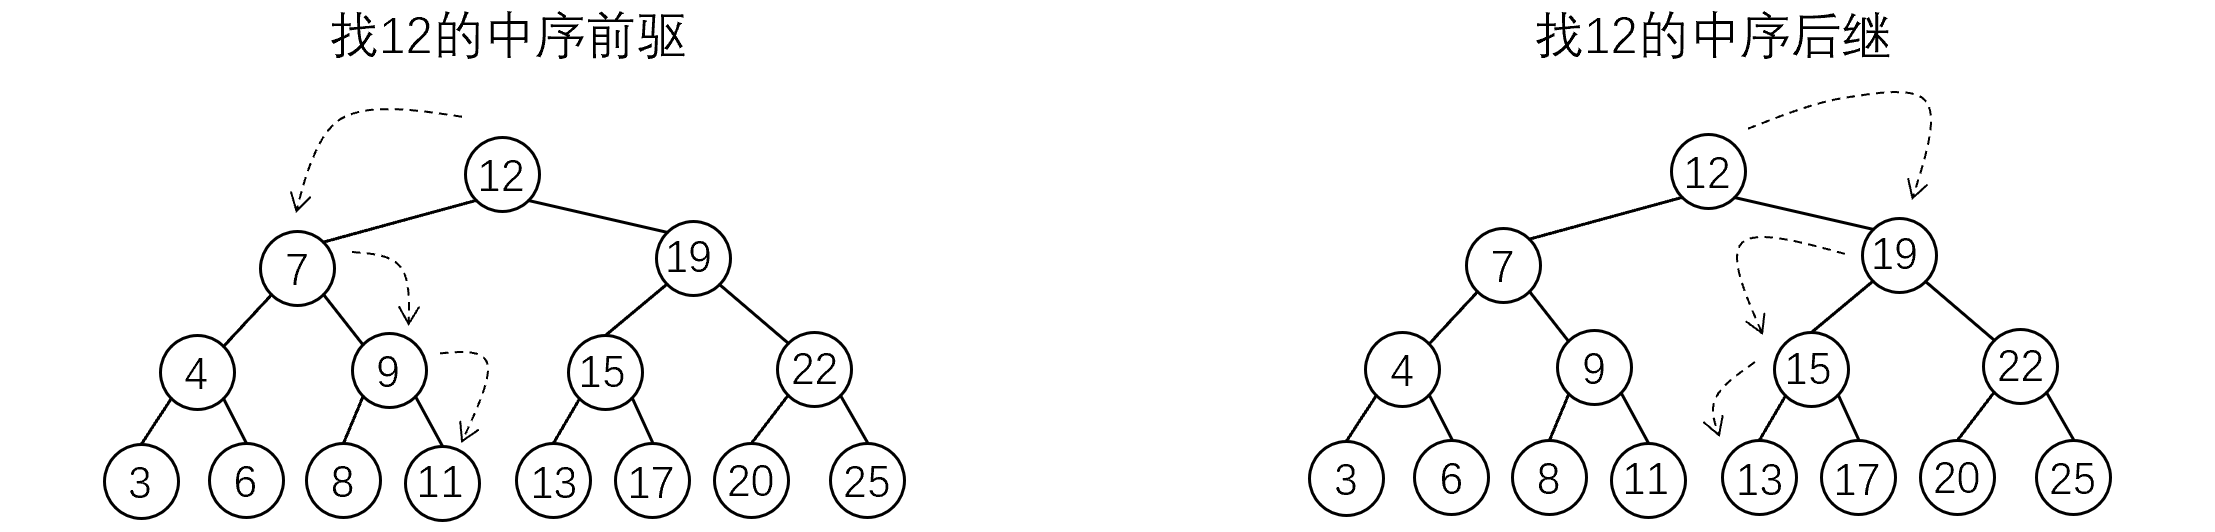
\includegraphics[width=0.89\textwidth]{assets/pics_and_ppts/ch4/中序前驱和中序后继.png}
    \caption{}
    \label{fig:中序前驱和中序后继}
\end{figure}

我们先给出两个辅助函数，用于寻找节点的中序前驱和中序后继：
\begin{cppcode}
// 寻找节点node的中序前驱
    BSTreeNode* FindInOrderPre(BSTreeNode* node) {
        // 该节点没有中序前驱，或中序前驱不存在于子树中
        if(node->lchild == NULL) {
            return NULL;
        }
        BSTreeNode* ret = node->lchild;
        while(ret->rchild != NULL) {
            ret = ret->rchild;
        }
        return ret;
        
    }
// 寻找节点node的中序后继
    BSTreeNode* FindInOrderPost(BSTreeNode* node) {
        // 该节点没有中序后继，或中序后继不存在于子树中
        if(node->rchild == NULL) {
            return NULL;
        }
        BSTreeNode* ret = node->rchild;
        while(ret->lchild != NULL) {
            ret = ret->lchild;
        }
        return ret;
        
    }
\end{cppcode}

根据上面的讨论，我们给出在二叉查找树T中删除关键字为e的节点的详细思路：

\Circled{1} 如果e大于当前节点，说明待删元素在右子树中，递归地在右子树中删除e；

\Circled{2} 如果e小于当前节点，类似地，递归地在左子树中删除e；

\Circled{3} 如果当前节点为空（NULL），说明树中不存在关键字为e的元素，直接返回即可；

\Circled{4} 如果e等于当前节点，说明找到了要删除的节点，进入删除操作：

a）若当前节点是叶节点，直接删除即可；

b）若当前节点有左孩子，那么可以在左子树中寻找节点的中序前驱pre，用pre的数据覆盖掉当前节点的数据，之后在左子树中删除节点pre；

c）若当前节点有右孩子，那么可以在右子树中寻找节点的中序后继post，用post的数据覆盖掉当前节点的数据，之后在右子树中删除节点post。

完整的删除代码如下所示：
\begin{cppcode}
// 在树root中，删除值为e的节点
    void DeleteBSTree(BSTreeNode* &root, ElemType e) {
        if(root == NULL) {
            return ;
        }
        if(e < root->data) {
            DeleteBSTree(root->lchild, e);
        }
        if(e > root->data) {
            DeleteBSTree(root->rchild, e);
        }
        if(e == root->data) {
            // root是叶节点
            if(root->lchild == NULL && root->rchild == NULL) {
                BSTreeNode* to_free = root;
                // root = NULL是为了改变链条，让其父节点的孩子指针指向NULL
                root = NULL;
                free(to_free);
            }
            // root不是叶节点
            else {
                // 有左子树
                if(root->lchild != NULL) {
                    // 若有左子树，则一定能找到中序前驱，所以pre一定不是NULL
                    BSTreeNode* pre = FindInOrderPre(root);
                    root->data = pre->data;
                    DeleteBSTree(root->lchild, pre->data);
                } 
                // 有右子树
                else if(root->rchild != NULL) {
                    BSTreeNode* post = FindInOrderPost(root);
                    root->data = post->data;
                    DeleteBSTree(root->rchild, post->data);
                }
            }
        }
    }
\end{cppcode}

\section{平衡二叉树}
在上一节中，可能你已经想到了，当我们使用序列{1,2,3,4,5,6,7,8,9}来构造一棵二叉查找树时，形成的树形是斜向右下的一条直线，高度为9。此时，二叉查找树实际上退化为
了一个线性表。许多具有类似结构特点的二叉查找树对查询、插入等操作带来的优化非常有限。

那么我们能不能在每次插入、删除元素后对树加以调整，让结构依然保持平衡？
例如当插入1到9时，对树进行如图\ref{fig:1到9插入调整过程}所示的调整。
\begin{figure}[htbp]
    \centering
    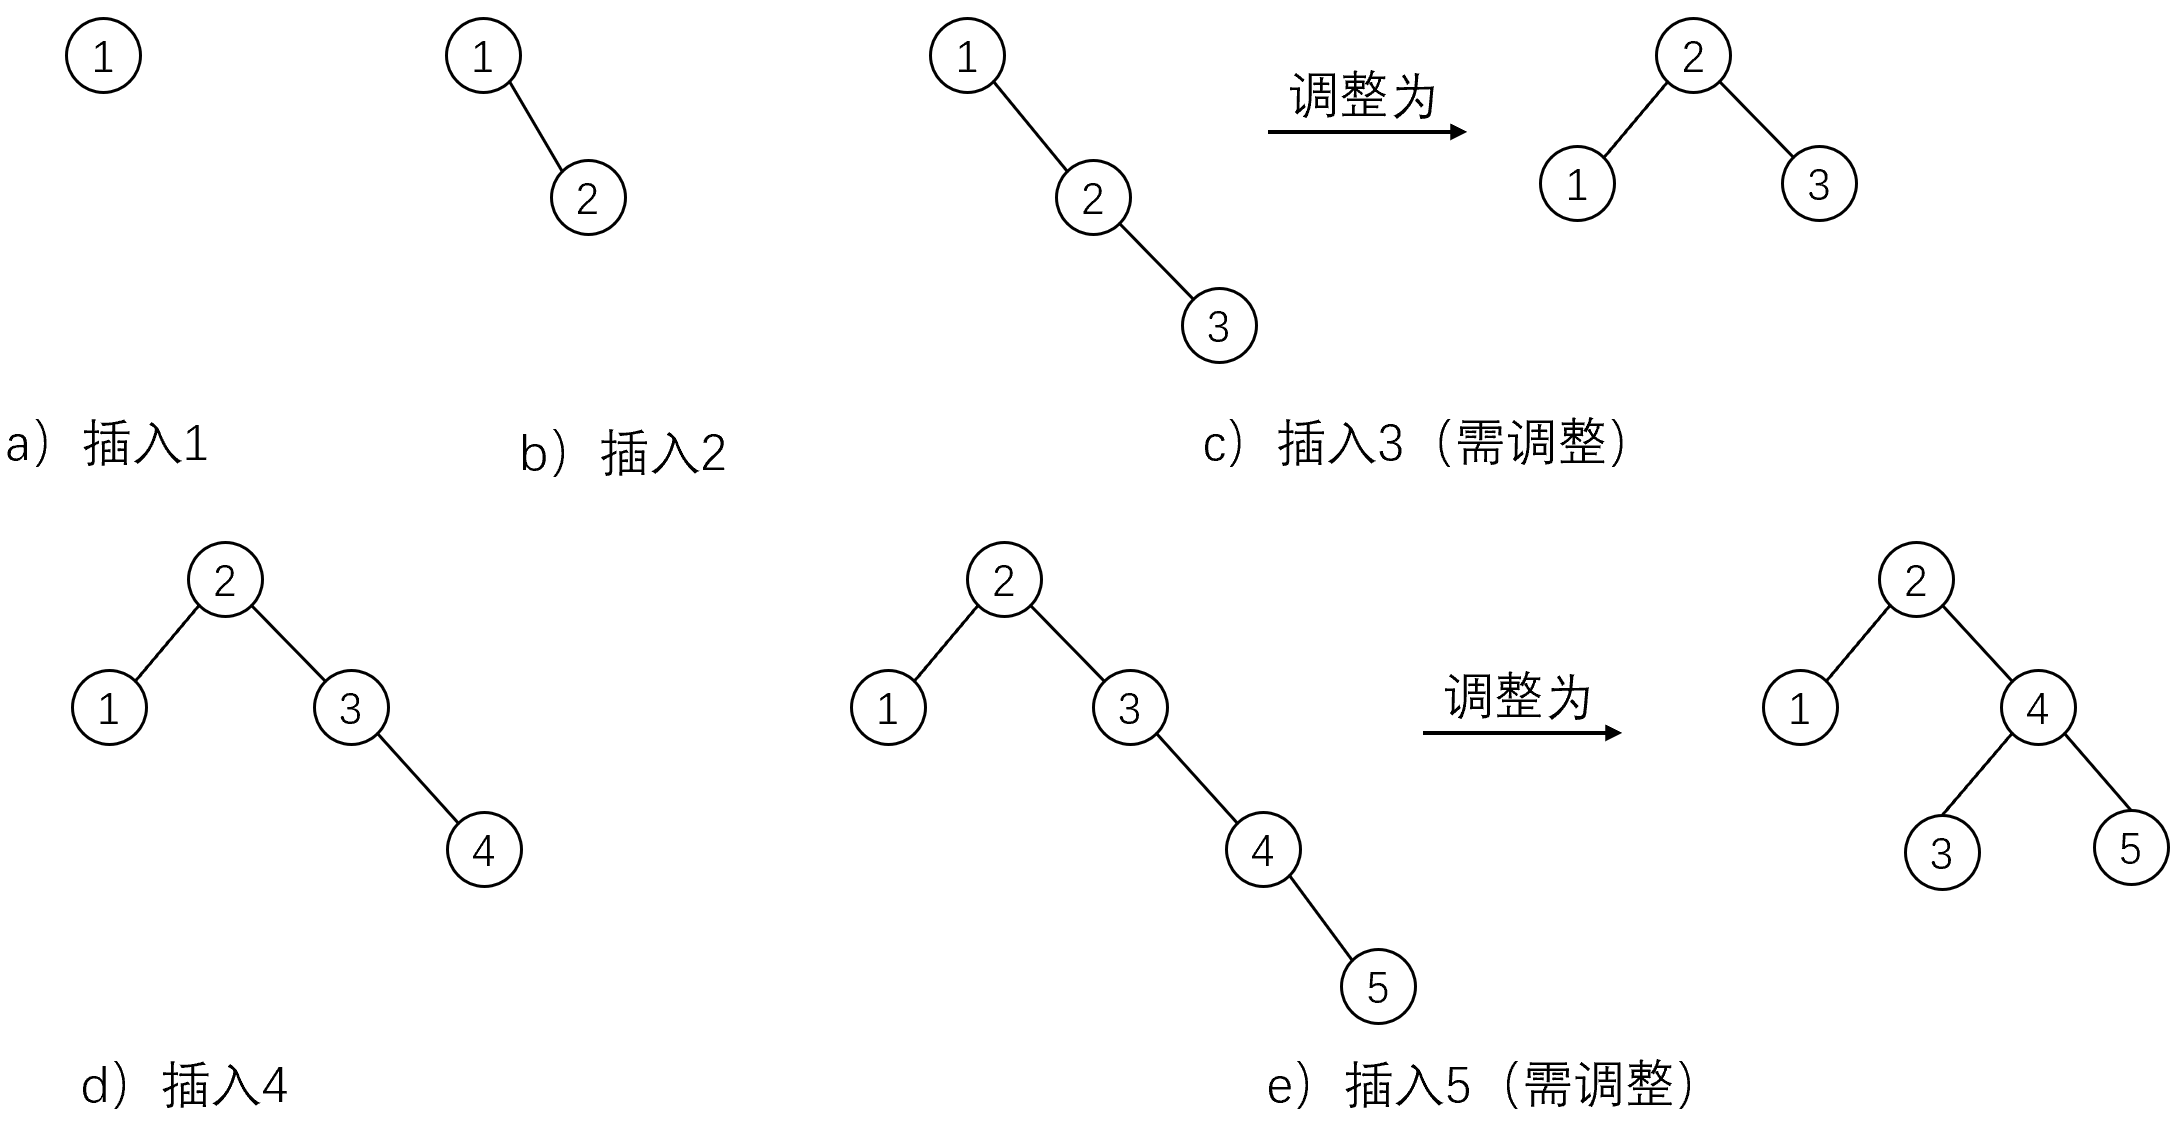
\includegraphics[width=1.0\textwidth]{assets/pics_and_ppts/ch4/1到9插入调整过程.png}
    \caption{}
    \label{fig:1到9插入调整过程}
\end{figure}
这样，二叉查找树始终能保持高效的，O(logn)级别的操作。基于这样的思想，两位先贤，名为G.M.\textbf{A}delse-\textbf{V}elskil以及
E.M.\textbf{L}andis提出了\term{平衡二叉树}，也被称为\term{AVL树}。AVL树是满足“平衡”要求的二叉查找树。所谓平衡，是指对树中任意节点来说，其左右子树的高度相差
不超过1。

对于一个节点，其左子树的高度减去右子树的高度，差值称为该节点的\term{平衡因子}（可以将节点理解为天平的中点，将其左右子树的高度分别理解为左右托盘的砝码数量）。
于是我们知道，\term{平衡二叉树要求树中任何一个节点的平衡因子的绝对值不超过1}。

图\ref{fig:1到9插入调整过程}中，c）调整前，节点1的左子树为空树，高度为0，右子树高度为2，因此节点1的
平衡因子为0-2=-2，左右子树高度相差2，不是平衡二叉树，而调整后，节点2、1、3的平衡因子都是0，因此是一棵平衡二叉树。
显然树中只要存在一个节点平衡因子的绝对值超过1，该树就不是平衡二叉树，因此我们需要一种手段记录每个节点的平衡因子。通常的做法并不是直接在节点的结构定义中记录平衡因子，
而是记录以当前节点为根节点的子树的高度：
\begin{cppcode}
    struct AVLTreeNode {
        ElemType data;
        AVLTreeNode* lchild;
        AVLTreeNode* rchild;
        int height;     // 以该节点为根的子树的高度。
    }
\end{cppcode}
\begin{notebox}{提示}
    height一定要理解为以该节点为根的子树的高度，为简洁不啰嗦，本节中我们表达为“节点高度”，但一定要将height理解为树的高度。
\end{notebox}

于是某节点的平衡因子就可以通过其左右子树高度之差计算得来。
\begin{cppcode}
// 返回节点root的平衡因子
    int GetBalance(AVLTreeNode* root) {
        int lheight;    // 左子树高度
        int rheight;    // 右子树高度

        // 注意不能直接通过root->lchild->height获取子树高度，若root没有左子树，应认为其左子树高度为0.
        if(root->lchild == NULL) {
            lheight = 0;
        }
        else {
            lheight = root->lchild->height;
        }
        if(root->rchild == NULL) {
            rheight = 0;
        }
        else {
            rheight = 0;
        }
        return lheight - rheight;
    }
\end{cppcode}
为了此处及后续诸多地方的代码书写简洁，我们封装一个函数来获取节点的高度：
\begin{cppcode}
    int GetHeight(AVLTreeNode* root) {
        if(root == NULL) return 0;
        return root->height;
    }
\end{cppcode}
于是获取平衡因子的函数就可以简单写成：
\begin{cppcode}
    int GetBalance(AVLTreeNode* root) {
        int lheight = GetHeight(root->lchild);
        int rheight = GetHeight(root->rchild);
        return lheight - rheight;
    }
\end{cppcode}

显然，当我们在平衡二叉树中插入一个新的节点之后，只需要更新该节点的所有\term{祖先节点}的height值，而非祖先的height是不受该新节点的影响的，无需更新。
如图\ref{fig:1到9插入调整过程}e），插入5后，节点1的height无需更新。由于节点root的height等于其左子树的height与右子树的height的较大值加一，
因此当新节点插入后，可以自下而上依次地更新新节点的每一个祖先节点的高度，通过如下函数：
\begin{cppcode}
    void UpdateHeight(AVLTreeNode* root) {
        int lheight = GetHeight(root->lchild);
        int rheight = GetHeight(root->rchild);
        root->height = max(lheight, rheight) + 1;
    }
\end{cppcode}

\begin{insightbox}
    实际上，有了前面二叉查找树插入操作的递归思想，你可能会想得到，“当新节点插入后，自下而上依次地更新每一个新节点的祖先节点的高度”，
    这个更新操作的时机就是在函数递归调用，找到正确的插入位置并插入元素之后再“回溯”到访问该节点的函数栈中时。大家可以结合后面平衡二叉树的插入代码体会。
\end{insightbox}


显然，平衡二叉树的查找操作与二叉查找树没有区别。而平衡二叉树的删除操作较为复杂，一般不做讨论。接下来我们就来重点研究平衡二叉树的插入操作。

\subsection{平衡二叉树的插入操作}
事实上图\ref{fig:1到9插入调整过程} c）所进行的调整，可以称为“进行了以节点1为根的\term{左旋}”。平衡二叉树的插入操作需要视情形对某些节点进行\term{左旋}或\term{右旋}。
我们先来看相关概念。
\begin{figure}[htbp]
    \centering
    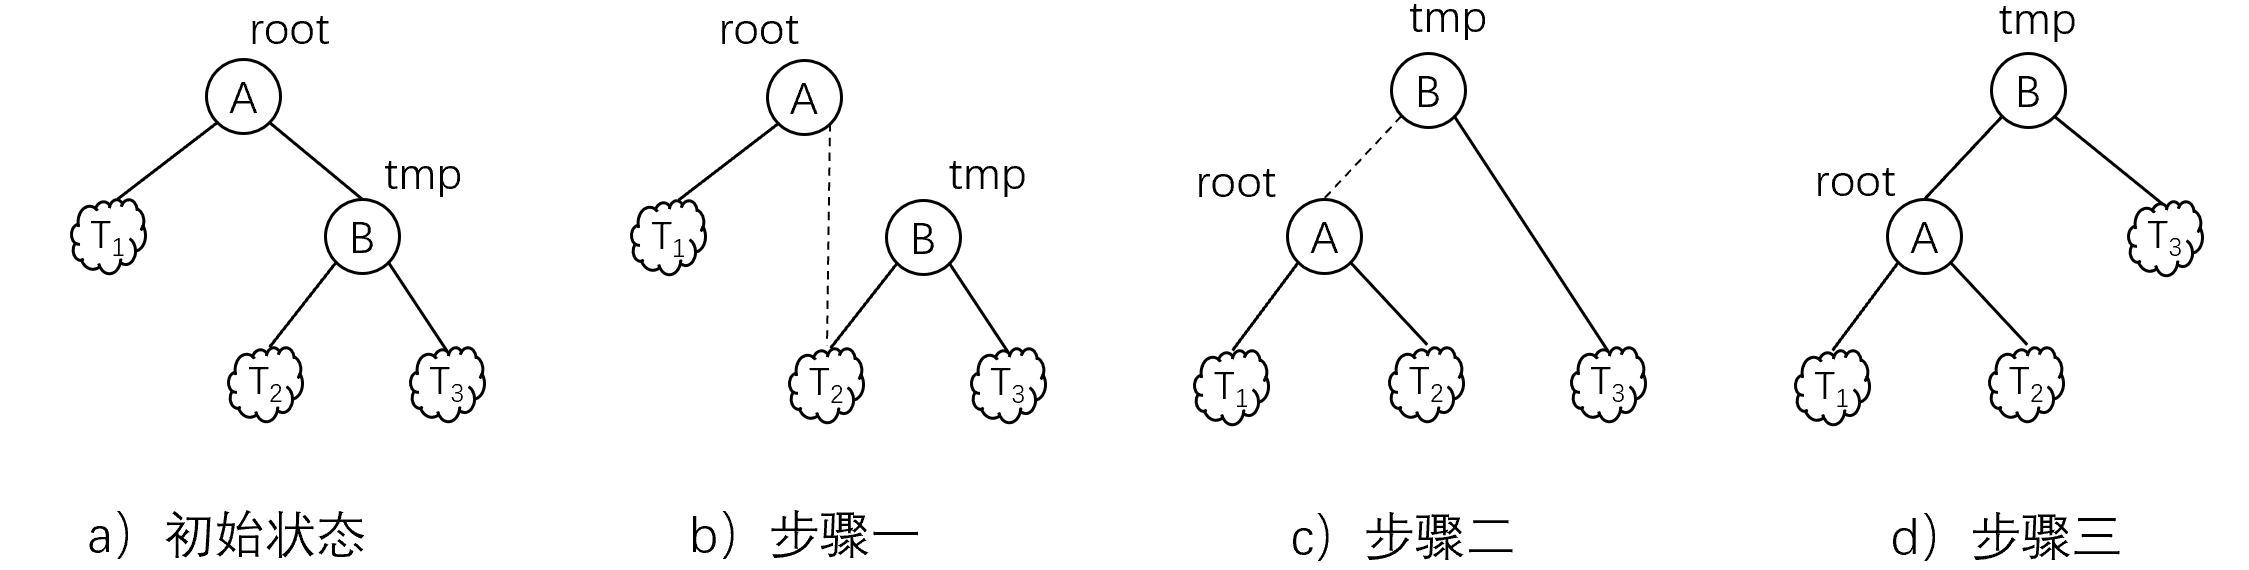
\includegraphics[width=0.91\textwidth]{assets/pics_and_ppts/ch4/左旋过程示意图.png}
    \caption{左旋过程示意图}
    \label{fig:左旋过程示意图}
\end{figure}
如图\ref{fig:左旋过程示意图}所示的过程将以节点A为根的子树进行了向左的旋转，具体过程如下：
\begin{enumerate}[label=\arabic*）]
    \item 让B的左子树$T_2$成为A的右子树；
    \item 让A成为B的左子树；
    \item 将根节点设定为节点B。
\end{enumerate}
像这样的，将原本的根节点A的右孩子“提升”为新的根节点，并且将A及其左子树“向左下沉”的操作，可以称为（以A为根节点的）\term{左旋}。
在后面的描述中我们简单地称为\textbf{对节点A左旋}。对root左旋的代码如下所示：
\begin{cppcode}
// 对节点root左旋
    void LRotate(AVLTreeNode* &root) {
        AVLTreeNode* tmp = root->rchild;
        root->rchild = tmp->lchild; // 步骤一
        tmp->lchild = root;     // 步骤二
        UpdateHeight(root);     // 先更新下层节点，在更新上层节点
        UpdateHeight(tmp);
        root = tmp;     // 步骤三
    }
\end{cppcode}
注意，$T_1$、$T_2$、$T_3$的height无需更新，因为旋转过程中这三棵树并未发生改变，他们的树高不变。A、B节点的height表示的是以A、B为根节点的子树的高度，这两棵子树
发生了变化，因此需要自下而上地先更新A的高度，再更新B的高度。

相应地，\term{右旋}是与左旋对称的过程，图\ref{fig:右旋过程示意图}展示了对节点B右旋的过程。
\begin{figure}[htbp]
    \centering
    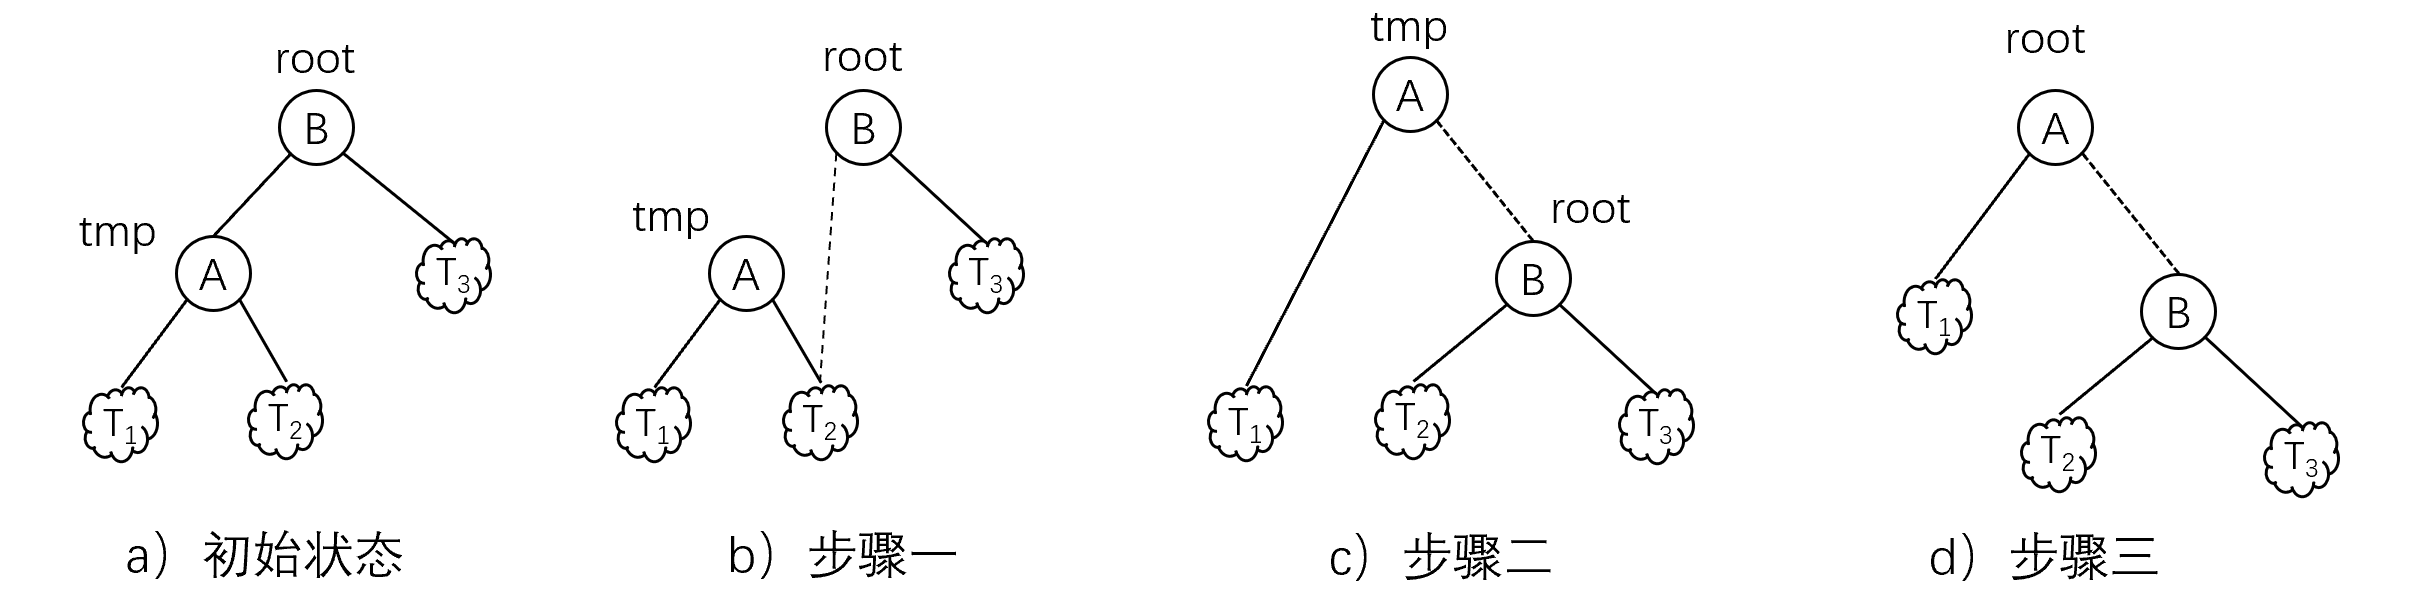
\includegraphics[width=0.91\textwidth]{assets/pics_and_ppts/ch4/右旋过程示意图.png}
    \caption{右旋过程示意图}
    \label{fig:右旋过程示意图}
\end{figure}
类似地可以写出代码：
\begin{cppcode}
// 对节点root右旋
    void RRotate(AVLTreeNode* &root) {
        AVLTreeNode* tmp = root->lchild;
        root->lchild = tmp->rchild;
        tmp->rchild = root;
        UpdateHeight(root);
        UpdateHeight(tmp);
        root = tmp;
    }
\end{cppcode}

以上介绍的左旋和右旋操作，正是用于失衡的调整。已经被证明，若失衡，我们只需要把新插入节点的所有祖先节点中，
最靠近新插入节点的那个失衡节点调整到正常，则路径上的所有节点就都会平衡。而最靠近新插入节点的失衡节点，其失衡的情形一定是
如图\ref{fig:四种失衡情形}所示四种情形之一。
\begin{figure}[htbp]
    \centering
    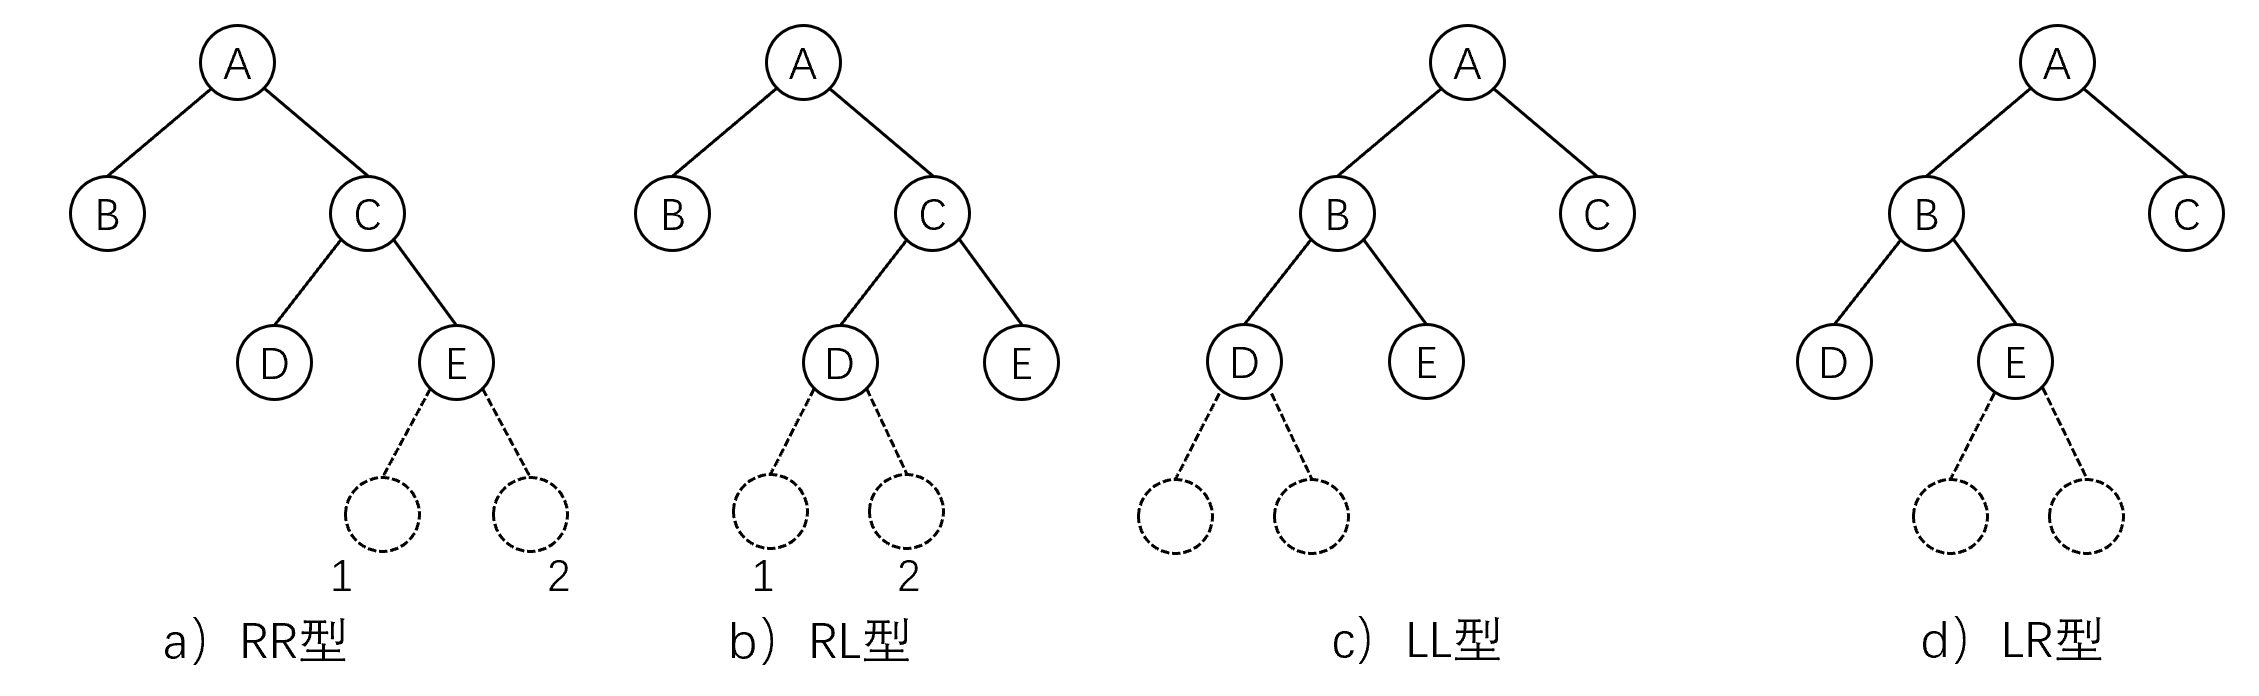
\includegraphics[width=0.85\textwidth]{assets/pics_and_ppts/ch4/四种失衡情形.png}
    \caption{四种失衡情形}
    \label{fig:四种失衡情形}

\end{figure}

图中用虚线表示新插入节点，根节点A表示最靠近新插入节点的失衡节点。若新插入节点在根节点的右子树（R）的右子树（R）中，则称这种失衡情形为\term{RR型}，
如a）所示；若新插入节点在根节点的右子树（R）的左子树（L）中，则称这种失衡情形为\term{RL型}，如b）所示；相应地，c）和d）分别被称为\term{LL型}
和\term{LR型}。

注意，对于a），无论插入位置是1还是2，都是在根节点的右子树的右子树（以E为根的子树）中，因此都叫做RR型；对于b），无论插入位置是1还是2，
都是在根节点的右子树的左子树（以D为根的子树）中，因此都叫做RL型。c）、d）情况类似。

一个很让人放心的事实是，这四种情形都可以通过若干次左旋或右旋的操作调整，从而重新达到平衡。先贤们将正确的做法传承了下来，见下。

\minisection{1.RR型}
对于RR型，直接将根节点（最靠近新插入节点的失衡节点）左旋即可。如图\ref{fig:RR型的调整方法}。

\begin{figure}[htbp]
    \centering
    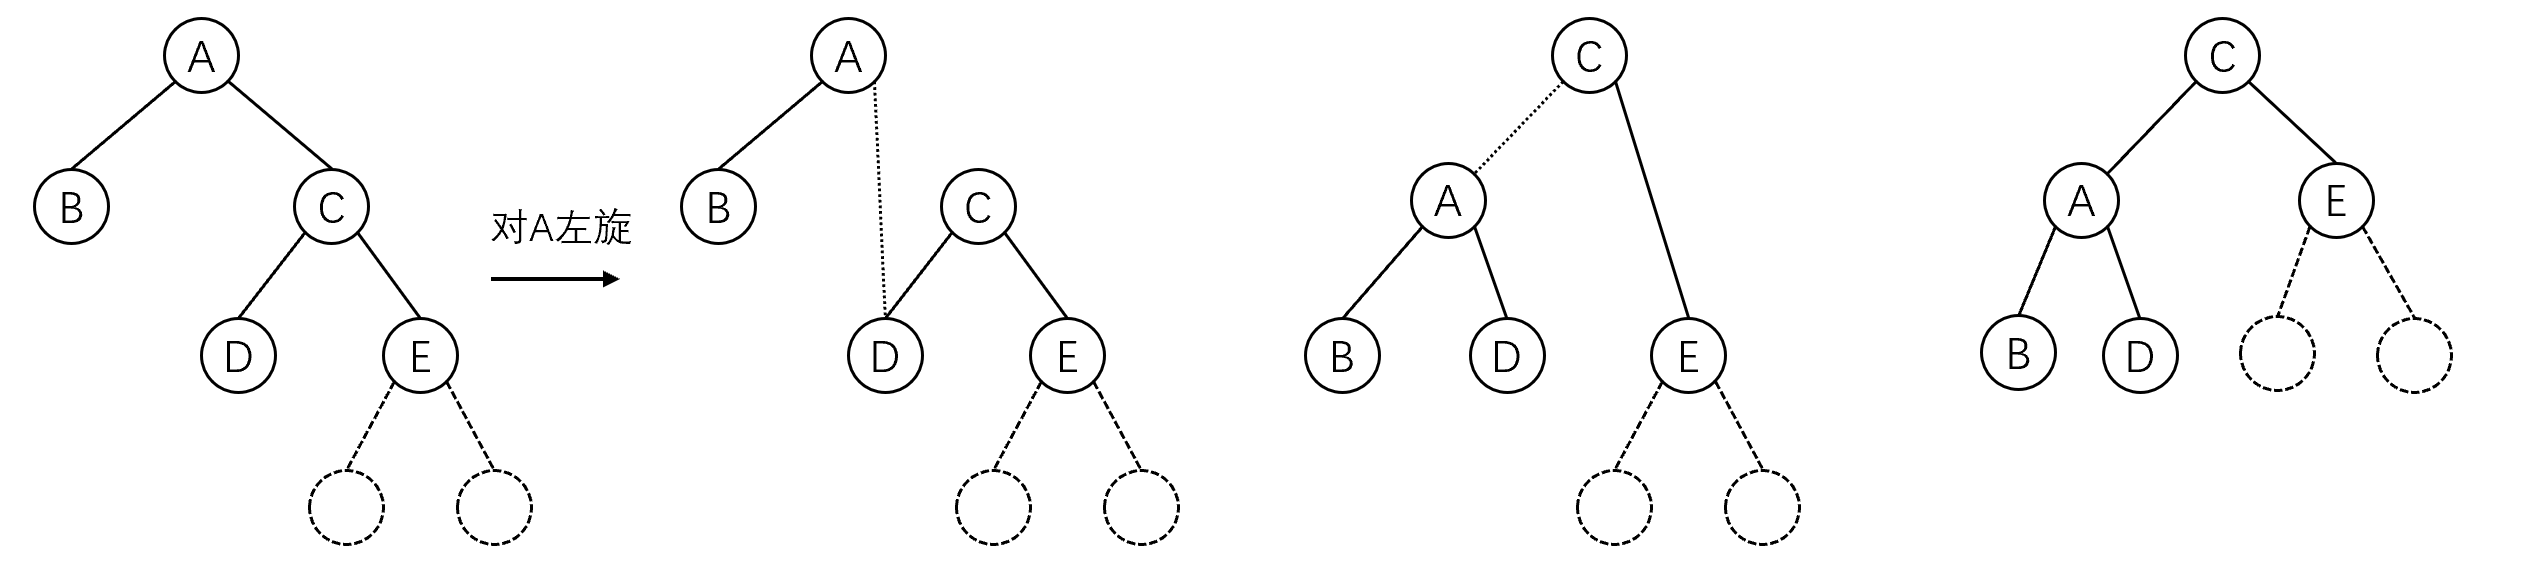
\includegraphics[width=0.99\textwidth]{assets/pics_and_ppts/ch4/RR型的调整方法.png}
    \caption{RR型的调整方法}
    \label{fig:RR型的调整方法}
\end{figure}

\minisection{2.RL型}
如图\ref{fig:RL型的调整方法}，对于RL型，可以先将根节点的右子树进行右旋（对C右旋），这样，就化归成了RR型失衡。再使用RR型的处理方式，对根节点左旋即可。
\begin{figure}[htbp]
    \centering
    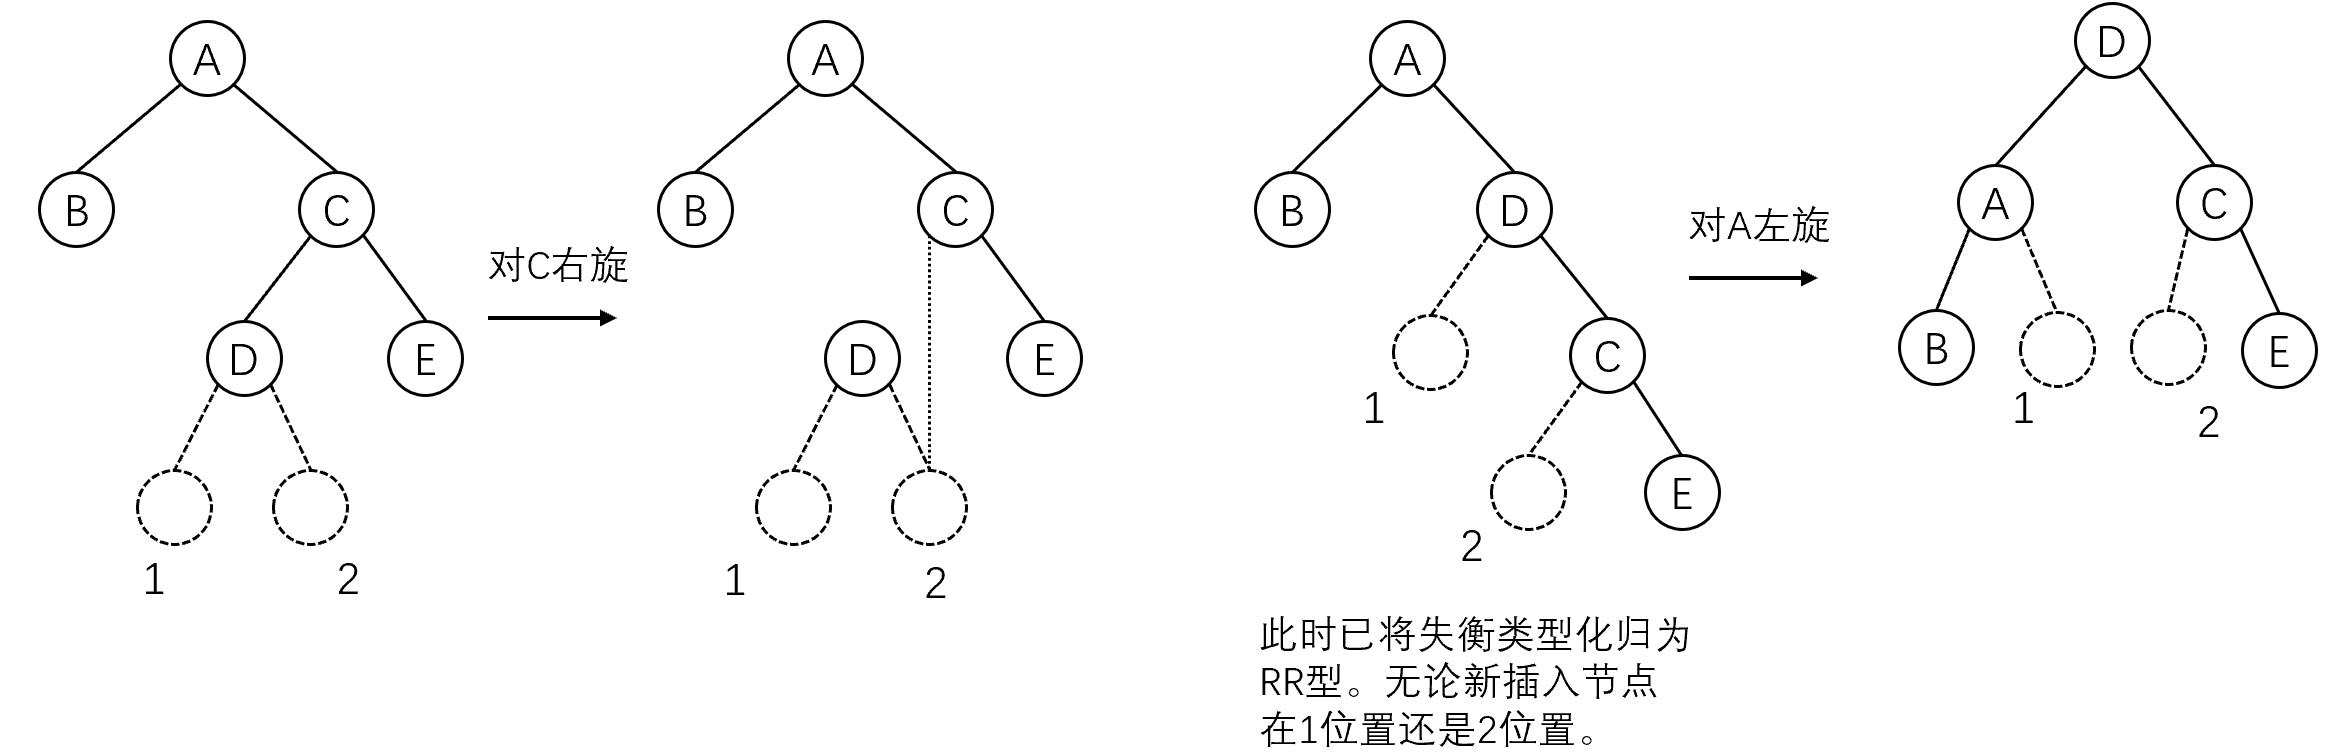
\includegraphics[width=0.99\textwidth]{assets/pics_and_ppts/ch4/RL型的调整方法.png}
    \caption{RL型的调整方法}
    \label{fig:RL型的调整方法}
\end{figure}

不难发现，LL型与RR型是对称的，LR型与RL型是对称的。因此处理LL型与LR型使用相应的对称的旋转方法即可。

\minisection{3.LL型}
LL型与RR型对称，使用与RR型对称的处理方法，直接将根节点右旋即可。如图\ref{fig:LL型的调整方法}。
\begin{figure}[htbp]
    \centering
    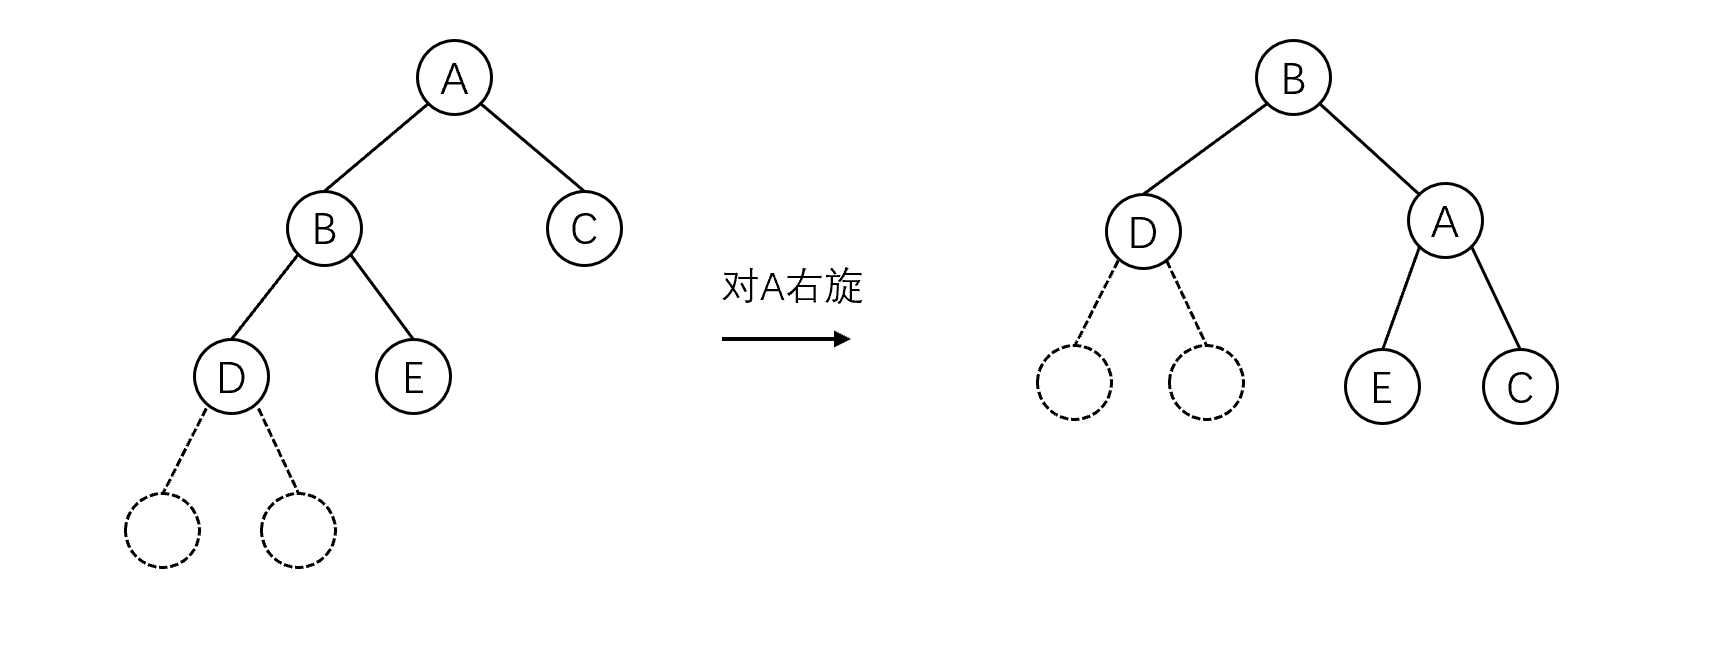
\includegraphics[width=0.81\textwidth]{assets/pics_and_ppts/ch4/LL型的调整方法.png}
    \caption{LL型的调整方法}
    \label{fig:LL型的调整方法}
\end{figure}


\minisection{4.LR型}
LR型与RL型对称。先将根节点的左子树左旋，再将根节点右旋。如图\ref{fig:LR型的调整方法}。
直接将根节点右旋即可。如图\ref{fig:LR型的调整方法}。
\begin{figure}[htbp]
    \centering
    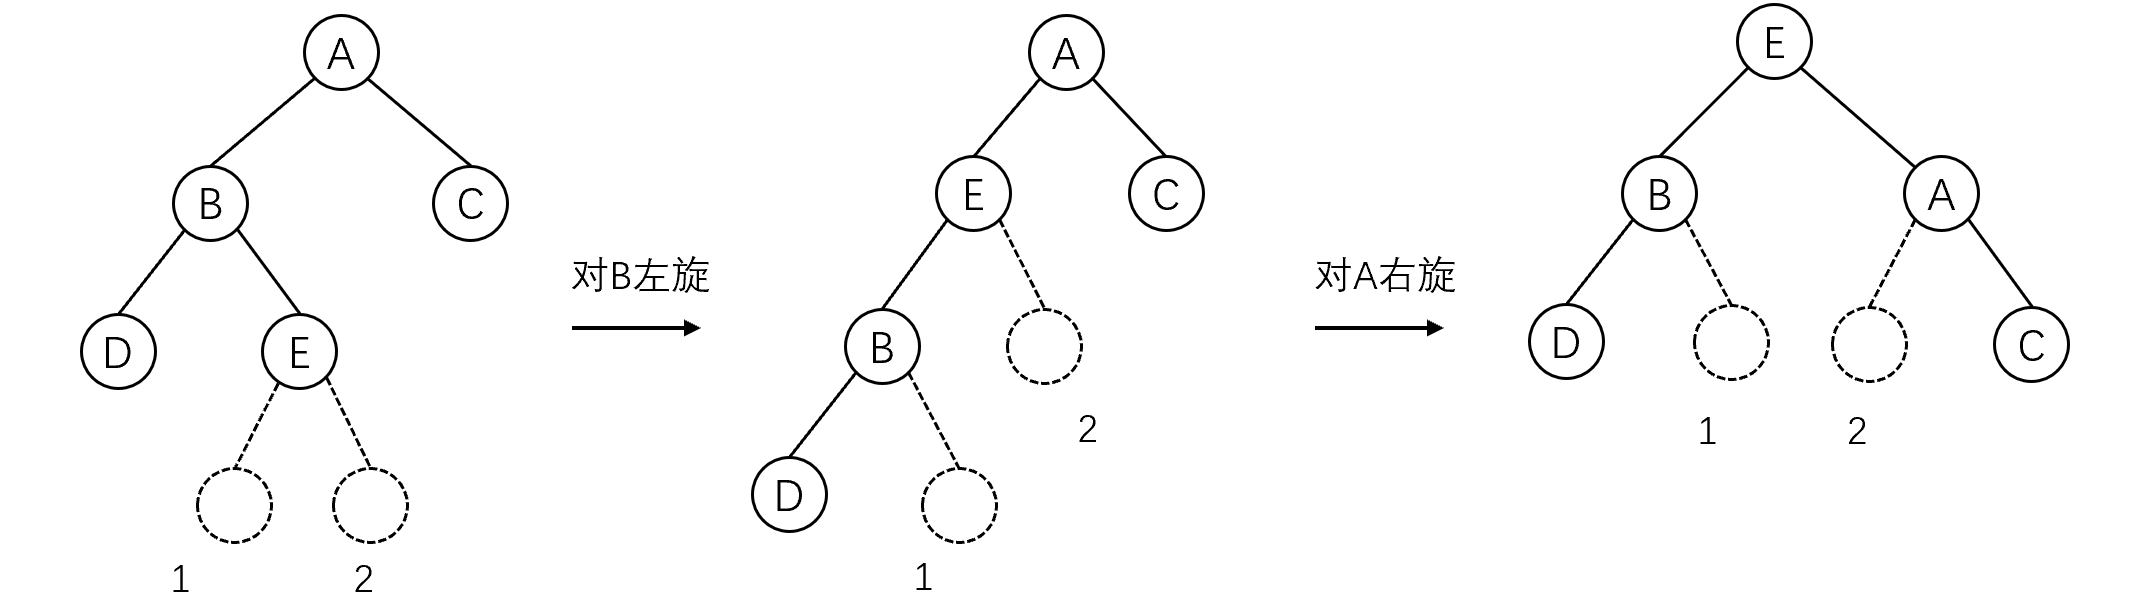
\includegraphics[width=0.93\textwidth]{assets/pics_and_ppts/ch4/LR型的调整方法.png}
    \caption{LR型的调整方法}
    \label{fig:LR型的调整方法}
\end{figure}


至此，我们来总结一下平衡二叉树的插入方法。首先，像普通二叉查找树的插入一样，沿着树递归向下找到插入位置，插入节点之后，
沿递归向上返回，判断每一个节点是否存在失衡，若失衡，判断失衡类型（LL、LR、RL、RR）并进行正确的调整即可。沿递归回去的路径判断失衡，第一个找到的失衡节点恰是
距离新插入节点最近的祖先节点。具体实现代码如下。

\begin{cppcode}
    void AVLTreeInsert(AVLTreeNode* &root, ElemType e) {
        // 找到了插入位置，插入
        if (root == NULL) {
            root = (AVLTreeNode*)malloc(sizeof(AVLTreeNode));
            root->data = e;
            root->height = 1;
            root->lchild = NULL;
            root->rchild = NULL;
            return;
        }
        // 关键字已存在，无需插入
        if(e == root->data) {
            return ;
        }
        // 在左子树中插入，只可能是LL型或LR型失衡
        if(e < root->data) {
            AVLTreeInsert(root->lchild, e);
            UpdateHeight(root);
            // 存在失衡
            if(GetBalance(root) == 2) {
                if(GetBalance(root->lchild) == 1) { // LL型失衡
                    RRotate(root);
                } else if(GetBalance(root->lchild) == -1) { // LR型失衡
                    LRotate(root->lchild);
                    RRotate(root);
                }
            }
        }
        // 在右子树中插入，只可能是RR型或RL型失衡
        else if(e > root->data) {
            AVLTreeInsert(root->rchild, e);
            UpdateHeight(root);
            // 存在失衡
            if(GetBalance(root) == -2) {
                if(GetBalance(root->rchild) == 1) { // RL型
                    RRotate(root->rchild);
                    LRotate(root);
                } else if(GetBalance(root->rchild) == -1) { // RR型
                    LRotate(root);
                }
            }
        }
    }
\end{cppcode}
以上代码的骨架和二叉查找树的插入操作一致，只不过在此基础上多了失衡判断和调整处理代码：
\begin{cppcode}
    void AVLTreeInsert(AVLTreeNode* &root, ElemType e) {
        // 找到了插入位置，插入
        if (root == NULL) {
            root = (AVLTreeNode*)malloc(sizeof(AVLTreeNode));
            root->data = e;
            root->height = 1;
            root->lchild = NULL;
            root->rchild = NULL;
            return;
        }
        // 关键字已存在，无需插入
        if(e == root->data) {
            return ;
        }
        // 在左子树中插入，只可能是LL型或LR型失衡
        if(e < root->data) {
            AVLTreeInsert(root->lchild, e);
            // UpdateHeight(root);
            // // 存在失衡
            // if(GetBalance(root) == 2) {
            //     if(GetBalance(root->lchild) == 1) { // LL型失衡
            //         RRotate(root);
            //     } else if(GetBalance(root->lchild) == -1) { // LR型失衡
            //         LRotate(root->lchild);
            //         RRotate(root);
            //     }
            // }
        }
        // 在右子树中插入，只可能是RR型或RL型失衡
        else if(e > root->data) {
            AVLTreeInsert(root->rchild, e);
            // UpdateHeight(root);
            // // 存在失衡
            // if(GetBalance(root) == -2) {
            //     if(GetBalance(root->rchild) == 1) { // RL型
            //         RRotate(root->rchild);
            //         LRotate(root);
            //     } else if(GetBalance(root->rchild) == -1) { // RR型
            //         LRotate(root);
            //     }
            // }
        }
    }
\end{cppcode}
图\ref{fig:平衡二叉树的插入过程}展示了在根节点12（平衡因子为-1）的平衡二叉树中，插入节点27的插入过程：
沿12、19、22、25、26一路递归向下，找到插入位置pos，插入节点27。此后递归回溯，回到26，重新计算节点26的height=max(0, 1)+1=2，
更新26的height为2。之后判断节点26的平衡因子，为0-1=-1，不失衡，递归继续向上返回到25，更新height为max(1, 2)+1=3，平衡因子为1-2=-1，
不失衡，递归继续向上返回，到22，更新height为4，平衡因子为1-3=-2，为RR型失衡，因此对22左旋，得到b）。继续返回19、12，函数结束。

\begin{figure}[htbp]
    \centering
    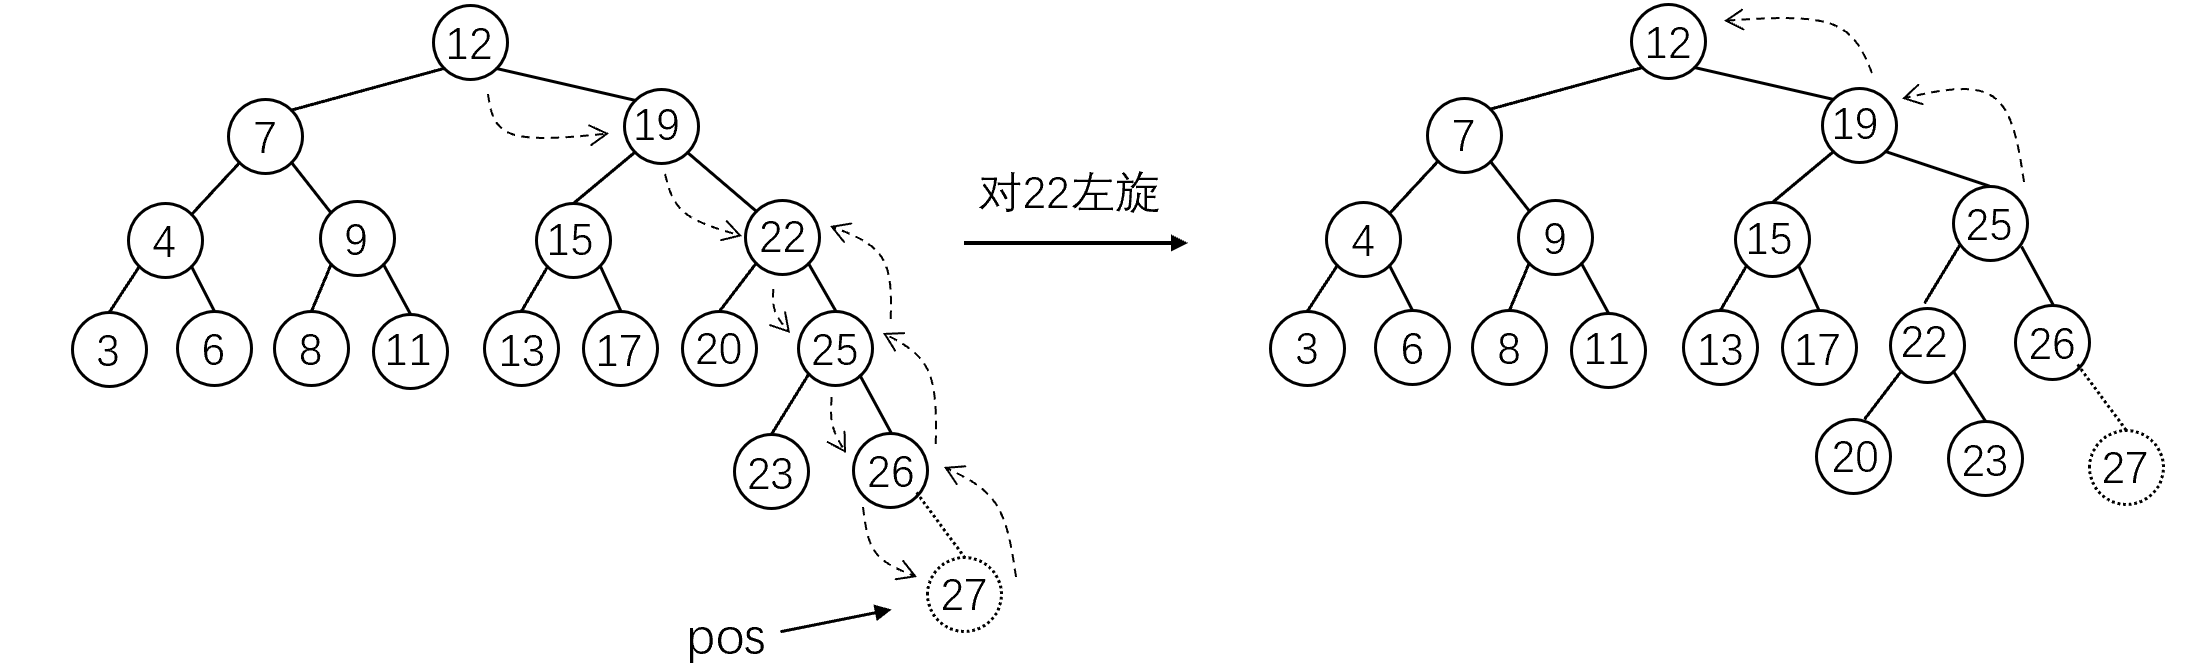
\includegraphics[width=0.90\textwidth]{assets/pics_and_ppts/ch4/平衡二叉树的插入过程.png}
    \caption{在平衡二叉树中插入节点27}
    \label{fig:平衡二叉树的插入过程}
\end{figure}

注意，在本节我们介绍二叉查找树以及平衡二叉树时，我们的定义是：左子树严格小于根节点、右子树严格大于根节点，即二叉树中不允许存在重复关键字。于是插入时，若
关键字已存在，直接返回。

\begin{insightbox}
    事实上，根据实际场景的不同需求，可能会需要允许重复关键字的树。绝大多数参考资料对此不做讨论，作为拓展，笔者给出一种较为简单的实现思路：\\

    在每个节点中增加一个链表，将所有相同关键字的数据存储起来：
    \begin{cppcode}
        struct node {
            int key;    // 关键字   
            LinkList<ElemType> datas;  // datas是一个链表，保存所有关键字为key的数据。
            node* lchild;
            node* rchild;
            int height;
        };
    \end{cppcode}
    这样，插入时，和链表中第一个节点比较即可。若相等，将新元素插入链表尾部。

\end{insightbox}
显然平衡二叉树的查找、插入操作的时间复杂度均为O(logn)。有了以上插入操作的实现，通过已有的n个元素构建一棵平衡二叉树，只需要依次将这n个元素插入树中即可。代码如下：
\begin{cppcode}
// 将存储在arr中的n个元素建立一棵平衡二叉树，返回树的根节点
    AVLTreeNode* CreateAVLTree(ElemType arr[], int n) {
        AVLTreeNode* root = NULL;
        for(int i=0; i<n; i++) {
            AVLTreeInsert(root, arr[i]);
        }
        return root;
    }
\end{cppcode}


\clearpage%%%%%%%%%%%%%%%%%%%%%%%%%%%%%%%%%%%%%%%%%%%%%%%%%%%%%%%%%%%%%%%%%%%%%%%%%%%%%%%%%%%%%%%%%%%%%%%%%%%%%%%%%%%%%%%%%%%%%%%%%%%%%%%%%%%%%%%%%%%%%
\begin{exercise}
1. [判断]二叉查找树，也称二叉排序树、二叉搜索树。\\

2. [判断]平衡二叉树一定都是二叉查找树。\\

3. （某年408真题）下列二叉排序树中，满足平衡二叉树定义的是\underline{\hspace{1cm}}\\
\begin{center}
    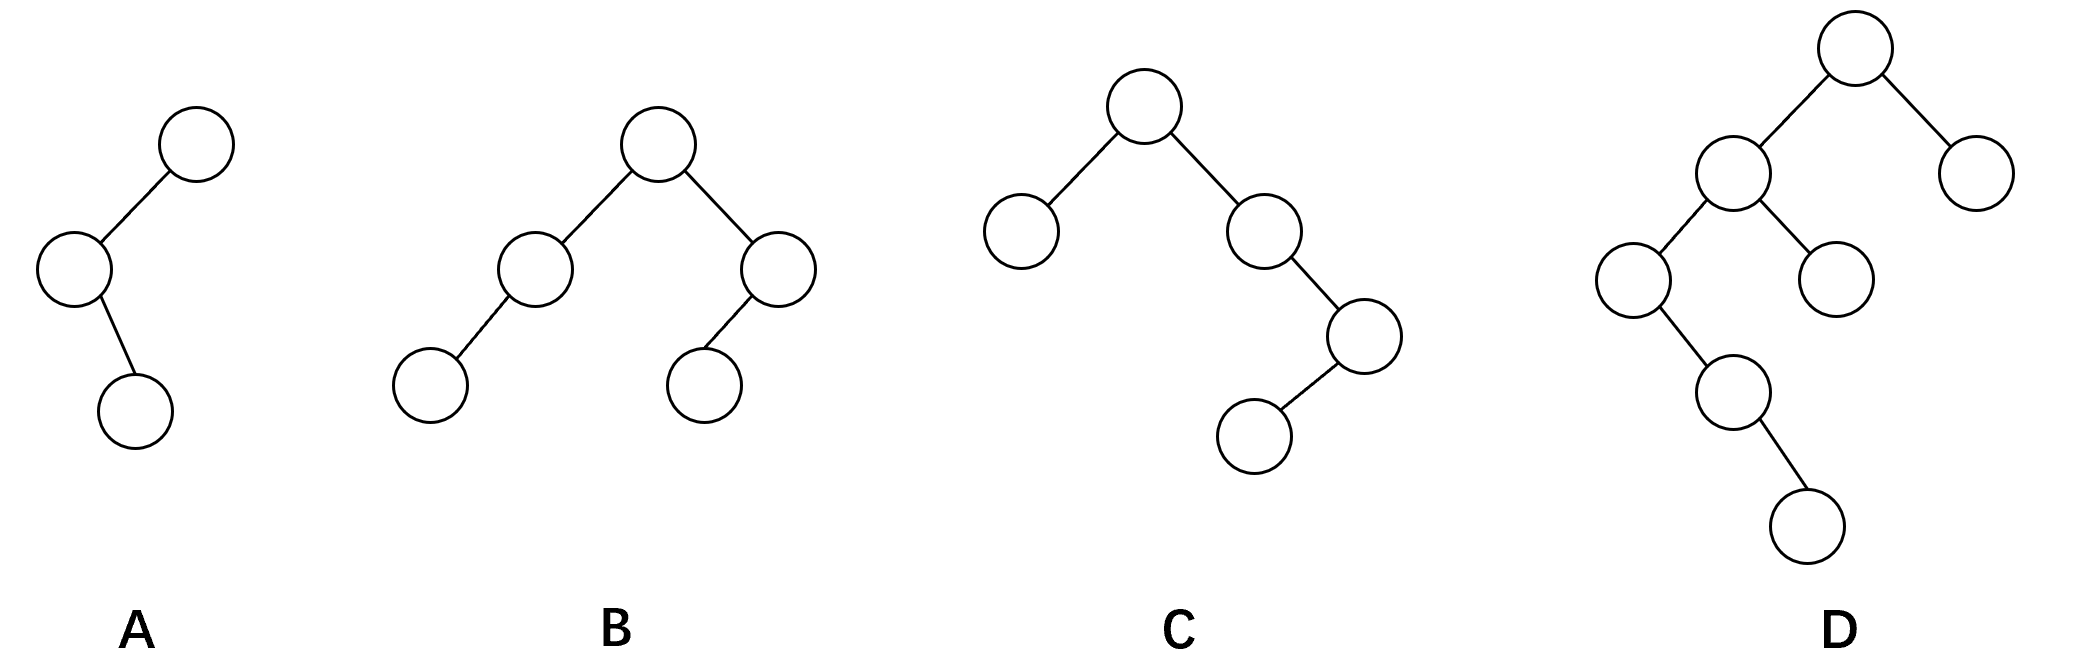
\includegraphics[width=0.81\textwidth]{assets/pics_and_ppts/ch4/09408_平衡二叉树定义.png}
\end{center}

\vspace{\baselineskip}

4. （某年408真题）对下列关键字序列，不可能构成二叉排序树中一条查找路径的是\underline{\hspace{1cm}}\\[0.5em]
\begin{tabular}{ll}
    A. 95, 22, 91, 24, 94, 71 & B. 92, 20, 91, 34, 88, 35\\
    C. 21, 89, 77, 29, 36, 38 & D. 12, 25, 71, 68, 33, 34\\
\end{tabular}

\vspace{\baselineskip}

5. （某年408真题）在下图所示的平衡二叉树中插入关键字48后得到一棵新的平衡二叉树，在新平衡二叉树中，关键字37所在节点的左、右子节点中保存的关键字分别是\underline{\hspace{1cm}}\\[0.5em]
\begin{center}
    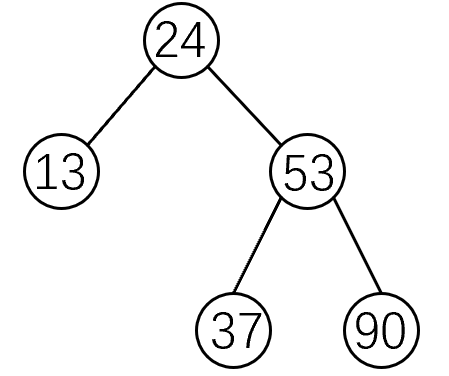
\includegraphics[width=0.21\textwidth]{assets/pics_and_ppts/ch4/10408_平衡二叉树插入后37的左右孩子值.png}
\end{center}

\begin{tabular}{llll}
    A. 13, 48 & B. 24, 48 & C. 24, 53 & D. 24, 90
\end{tabular}

\vspace{\baselineskip}

6. （某年408真题）下列给定的关键字输入序列中，不能生成如图所示的二叉排序树的是\underline{\hspace{1cm}}\\[0.5em]
\begin{center}
    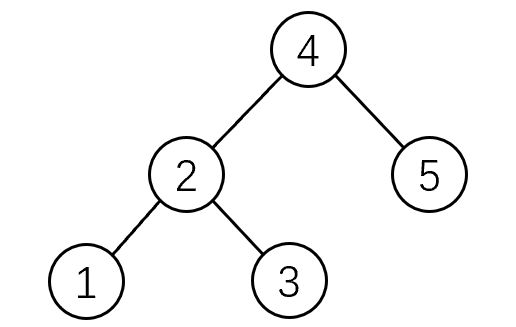
\includegraphics[width=0.22\textwidth]{assets/pics_and_ppts/ch4/20408哪一个序列不能生成图示二叉排序树.png}
\end{center}

\noindent A. 4, 5, 2, 1, 3\\
B. 4, 5, 1, 2, 3\\
C. 4, 2, 5, 3, 1\\
D. 4, 2, 1, 3, 5\\

7. (提示：本题是一个比较经典的问题，但有一定思维门槛。建议大家根据自身需求选择直接跳过，或思考1-2分钟，若无思路，可以直接研读参考答案，学会最近公共祖先的求法，并获得一定启发即可。)\\

请你设计一个算法，给定任意一棵二叉树以及两个关键字a和b，返回树中a和b的最近公共祖先。假设关键字类型为int。保证树中无重复关键字并且a、b一定都存在于树中。
节点自身也被认为是自身的祖先。
如图所示的树中，4、5的最近公共祖先为2；4、3的最近公共祖先为1；2、5的最近公共祖先被认为是2。
\begin{center}
    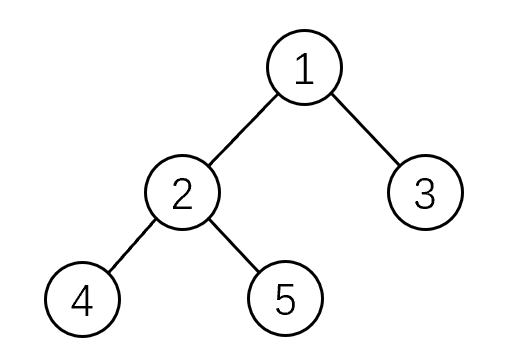
\includegraphics[width=0.25\textwidth]{assets/pics_and_ppts/ch4/习题_寻找公共祖先答案图.png}
\end{center}

\begin{cppcode}
    struct node {
        int key;
        node* lchild;
        node* rchild;  
    };

    node* LowestCommonAncestor(node* root, int a, int b) {

    }
\end{cppcode}

\vspace{\baselineskip}

8. 若上一题并非任意二叉树，而是一棵二叉搜索树，其他条件不变，则可解上题的代码一定可解本题吗？代码会有哪些优化空间吗？
若你研究了上一题的思想，可以思考写出本题的代码。\\

9. 请你设计一个算法，查找二叉搜索树中第k小的元素。
\begin{cppcode}
// 返回二叉搜索树root中第k小的元素
    int kthSmallest(node* root, int k) {

    }
\end{cppcode}

\vspace{\baselineskip}

10. （某年408真题）已知非空二叉树T的节点值均为正整数，采用顺序存储方式保存，数据结构定义如下：
\begin{cppcode}
    typedef struct {                // MAX_SIZE为已定义常量
        int SqBiTNode[MAX_SIZE];    // 保存二叉树节点值得数组
        int ElemNum;                // 实际占用的数组元素个数
    }SqBiTree;
\end{cppcode}
T中不存在的节点在数组SqBitNode中用-1表示。例如，对于下图所示得两棵非空二叉树$T_1$和$T_2$，
\begin{center}
    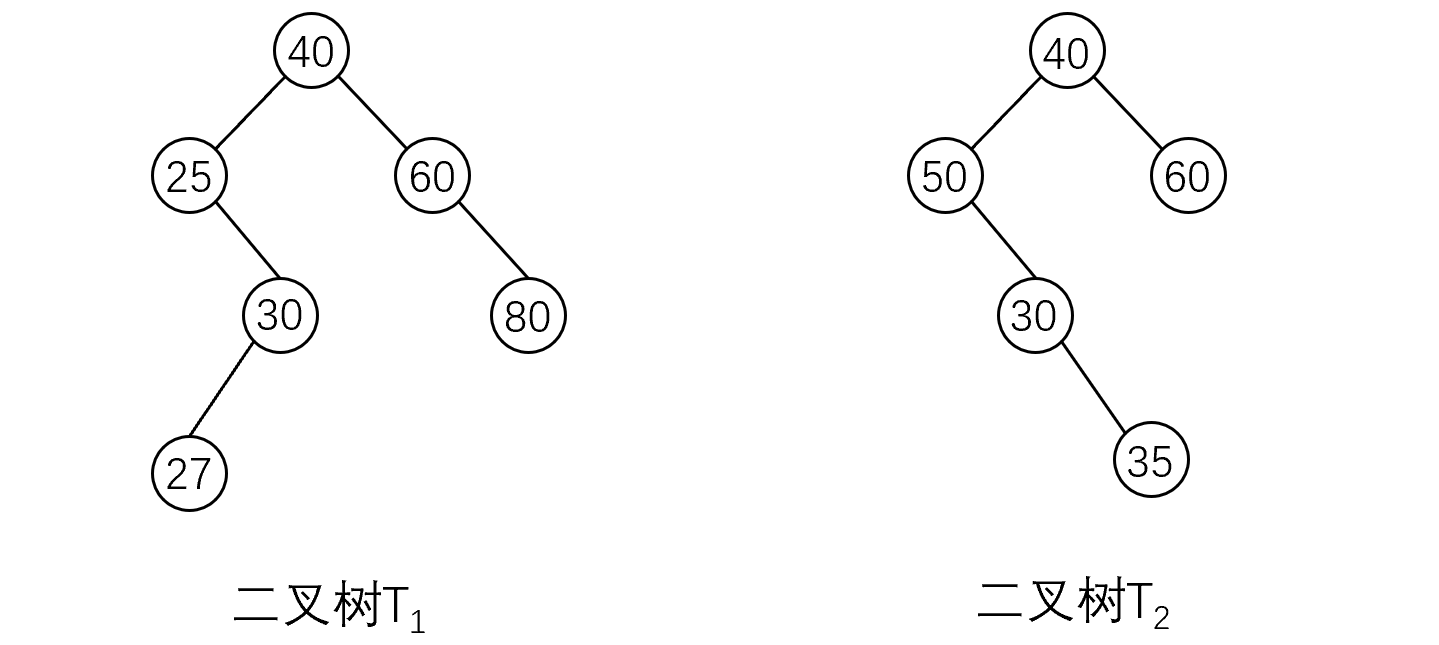
\includegraphics[width=0.71\textwidth]{assets/pics_and_ppts/ch4/22408T1T2.png}
\end{center}
$T_1$的存储结果如下：
\begin{center}
    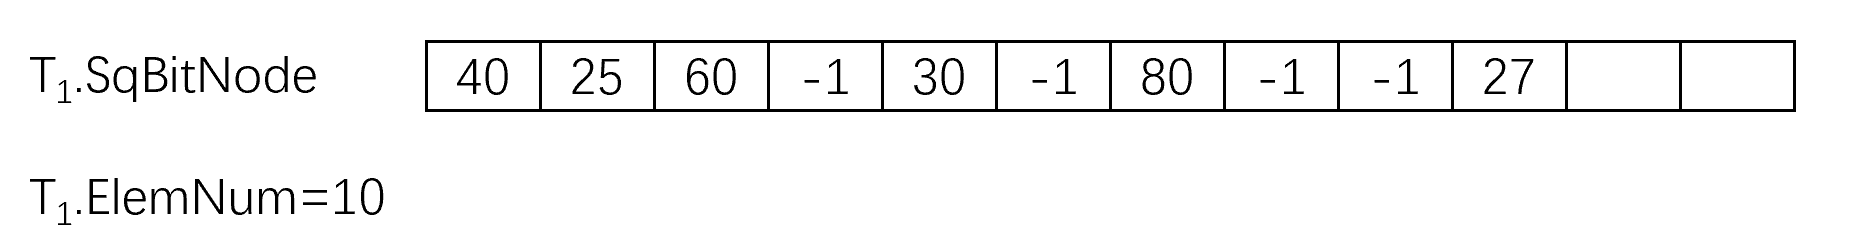
\includegraphics[width=0.71\textwidth]{assets/pics_and_ppts/ch4/22408T1存储.png}
\end{center}
$T_2$的存储结果如下：
\begin{center}
    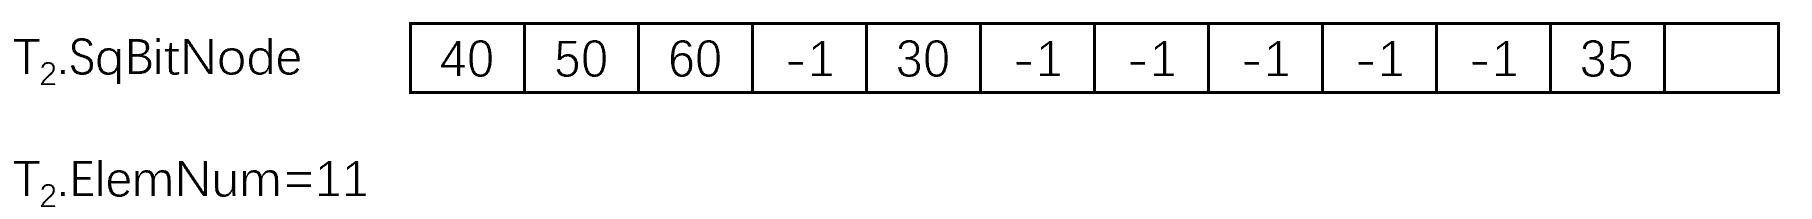
\includegraphics[width=0.76\textwidth]{assets/pics_and_ppts/ch4/22408T2存储.png}
\end{center}

请设计一个尽可能高效的算法，判定一棵采用这种方式存储的二叉树是否为二叉搜索树，若是，则返回true，否则，返回false，要求：

1）给出算法的基本设计思想；

2）根据设计思想，采用C或者C++语言描述算法，关键之处给出注释。

\end{exercise}

\clearpage



\begin{exerciseanswer}
1. 正确。\\

2. 正确。\\

3. 选B。A、C、D均存在平衡因子的绝对值大于1的节点，如图所示。\\
\begin{center}
    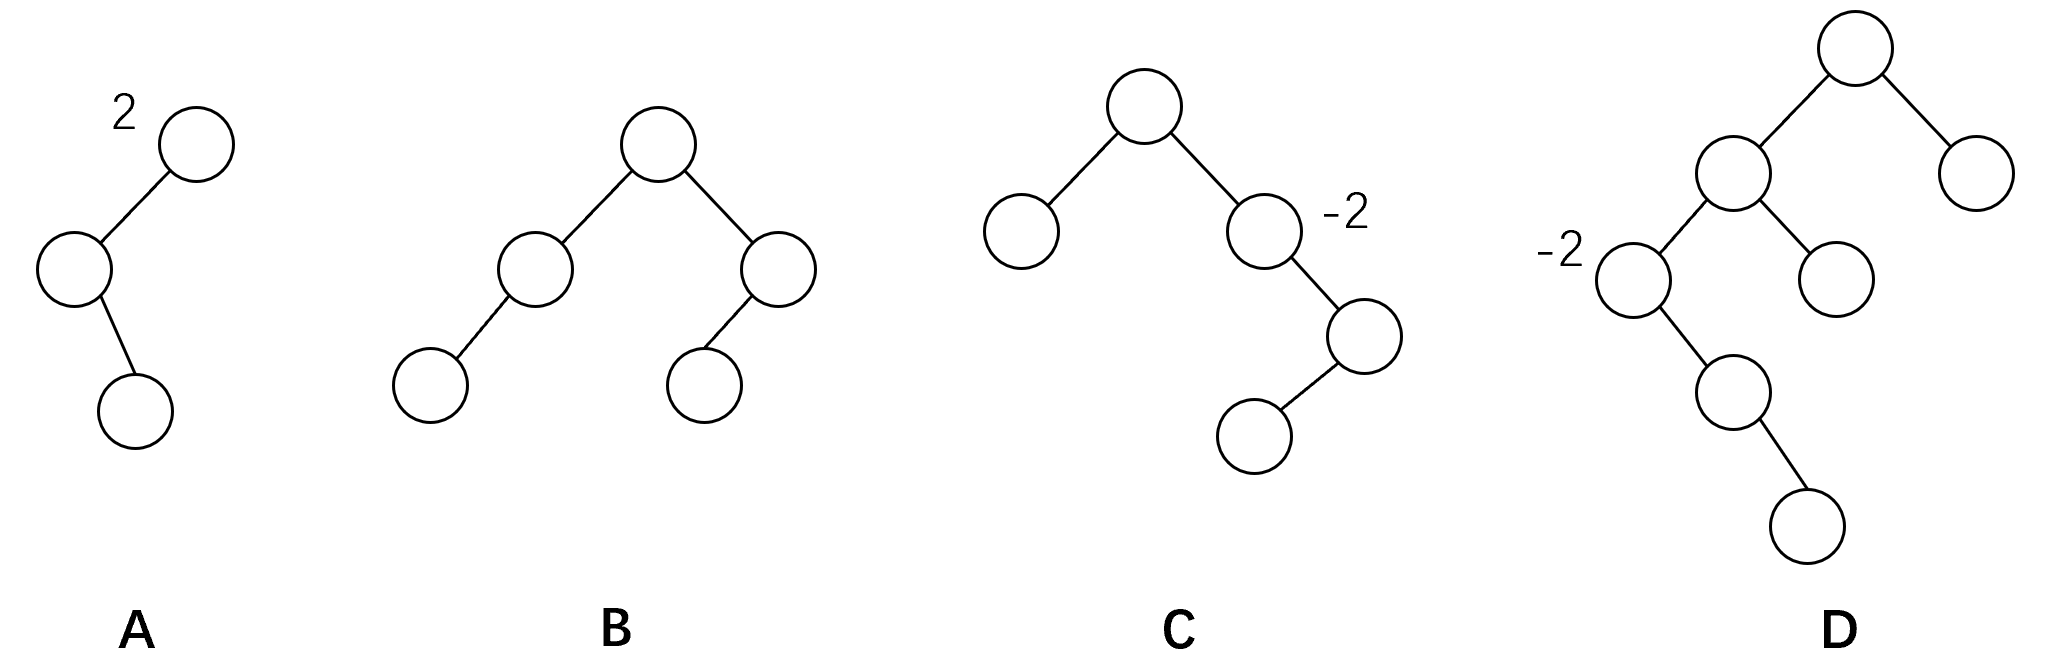
\includegraphics[width=0.80\textwidth]{assets/pics_and_ppts/ch4/09408_平衡二叉树定义答案图.png}
\end{center}

4. 选A。各选项查找过程如下图所示：
\begin{center}
    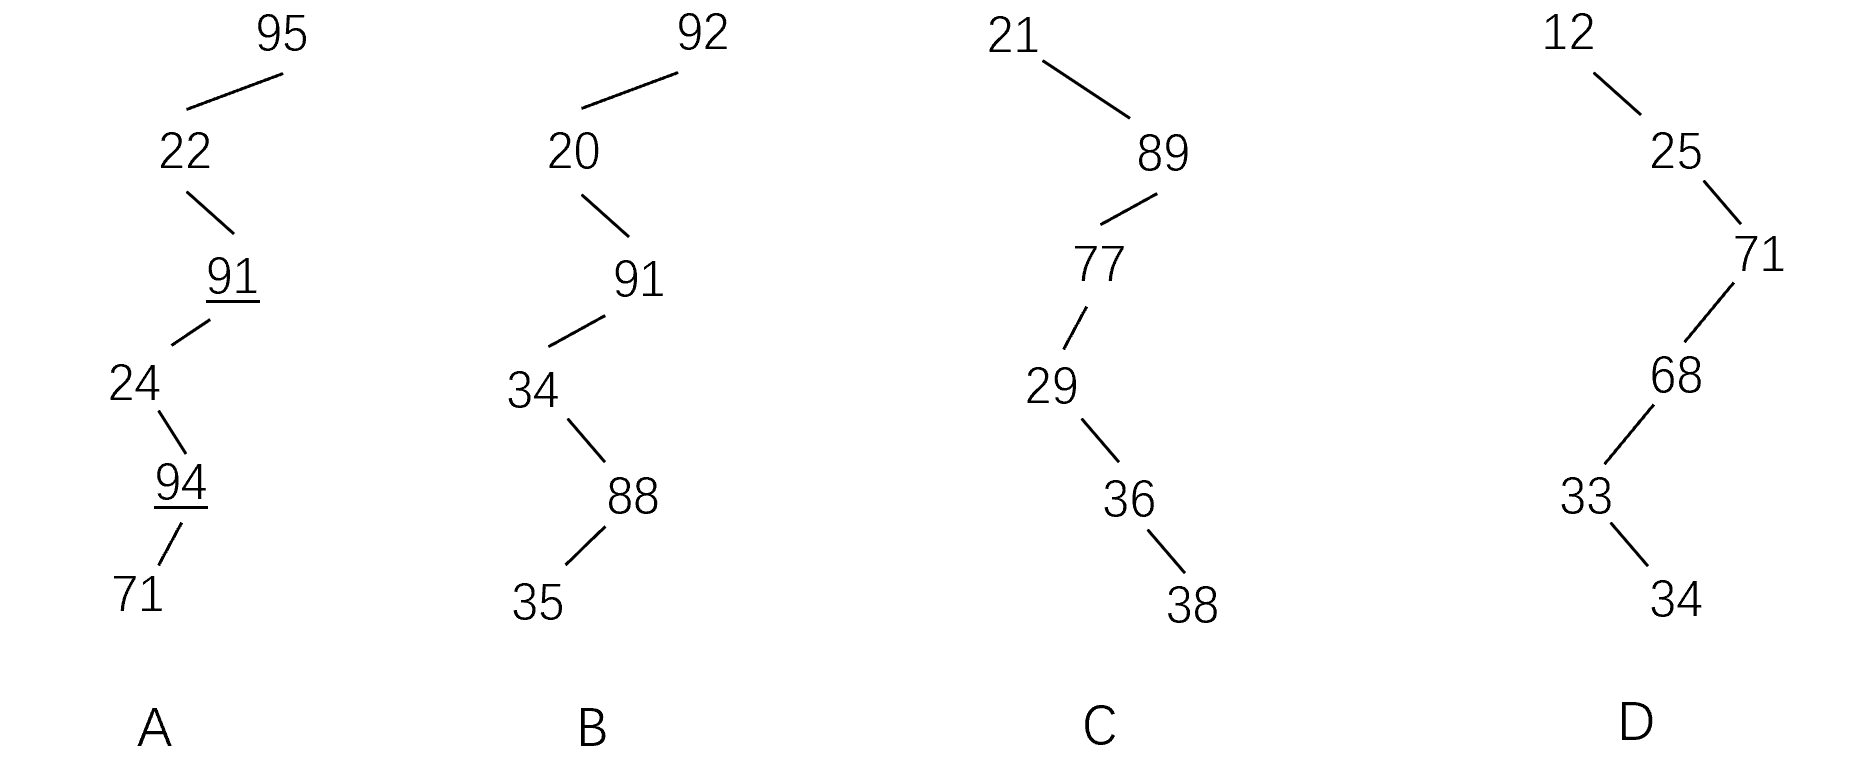
\includegraphics[width=0.8\textwidth]{assets/pics_and_ppts/ch4/11408_二叉查找树查找路径答案图.png}
\end{center}
图A，91的左子树出现了94，大于91，因此不可能是二叉排序树的查找路径。    \\

5. 选C。插入48后，据新插入节点48最近的失衡节点为24（根节点），平衡因子为1-3=-2，为RL型失衡。先对53右旋，再对24左旋，调整后37的左、右孩子分别是24、53，如下图所示。
\begin{center}
    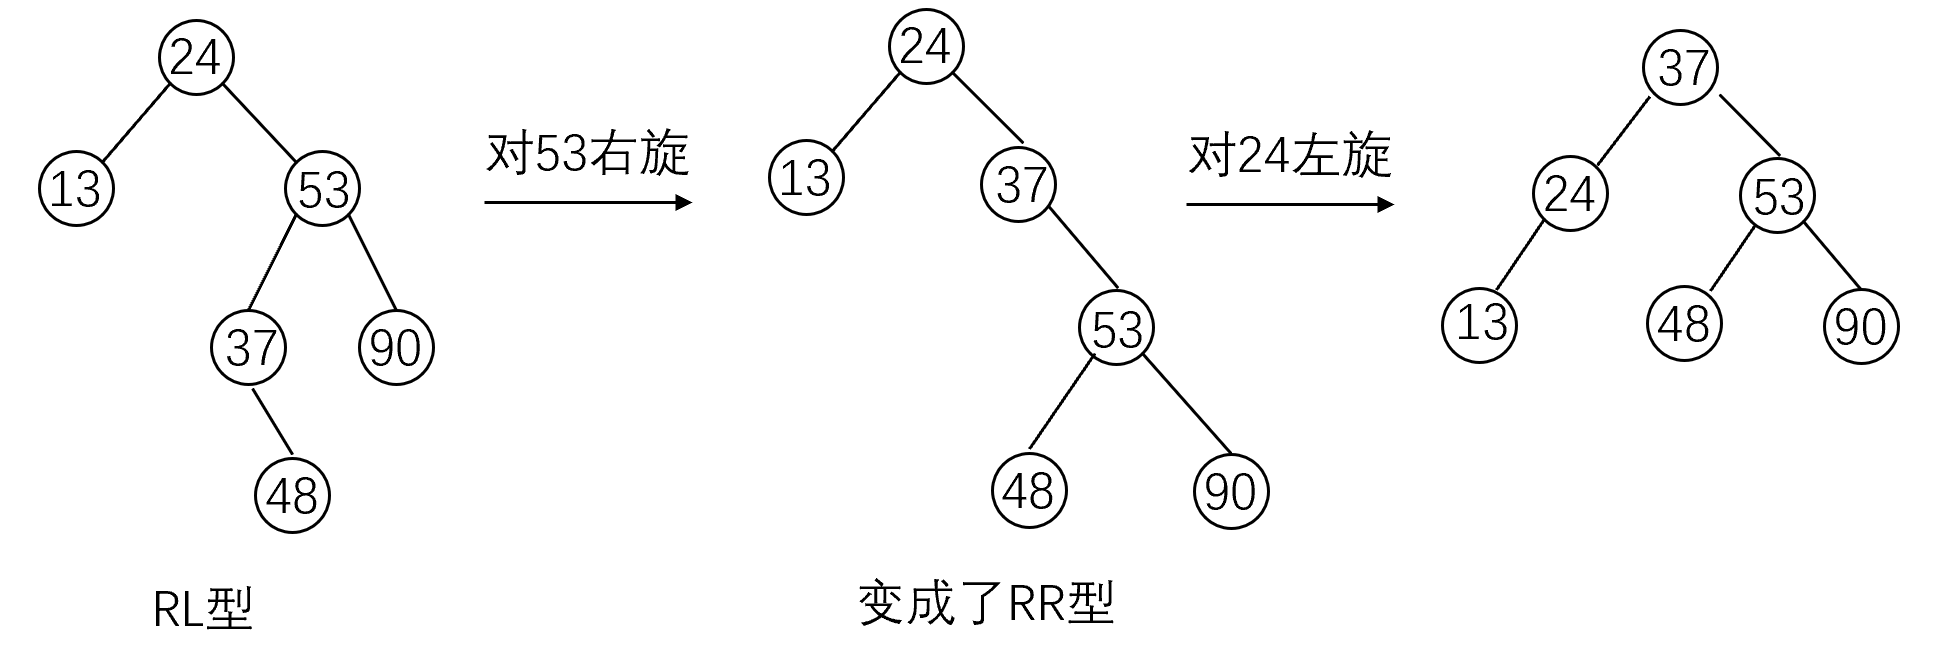
\includegraphics[width=0.81\textwidth]{assets/pics_and_ppts/ch4/10408_平衡二叉树插入后37的左右孩子值答案图.png}
\end{center}

\vspace{\baselineskip}

6. 选B。B项插入序列生成的二叉排序树如图所示：
\begin{center}
    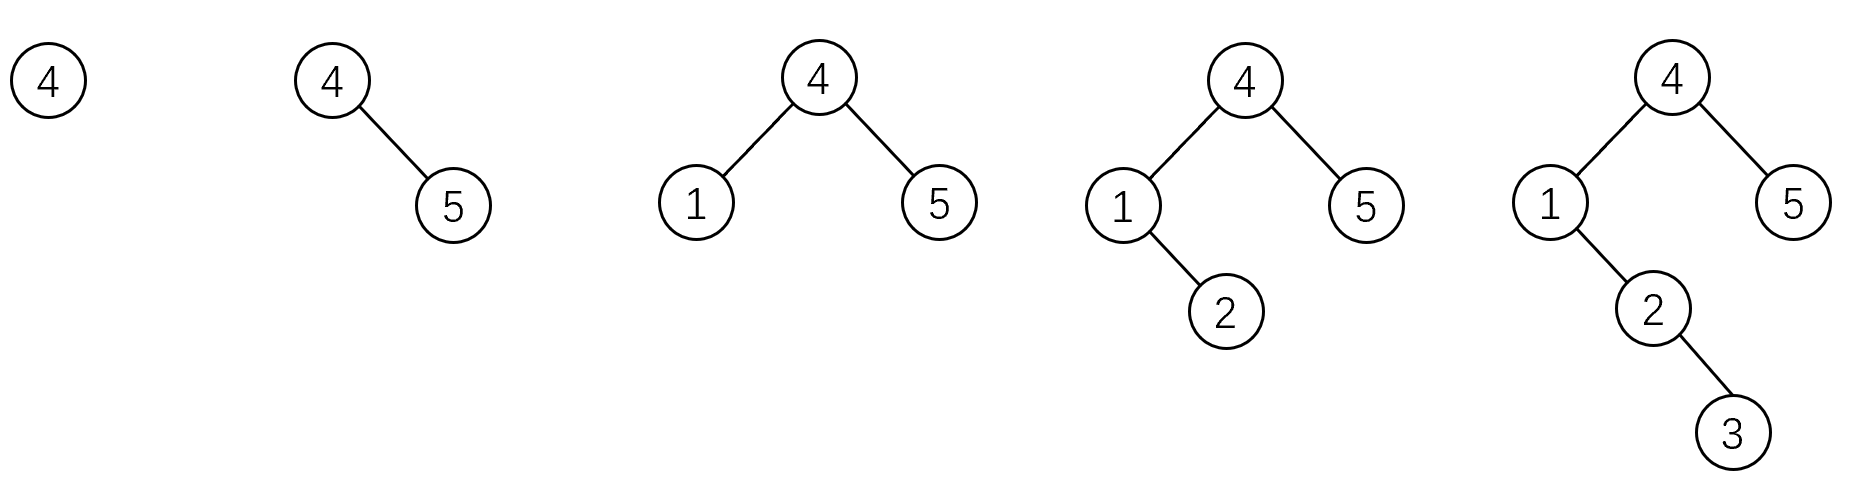
\includegraphics[width=0.78\textwidth]{assets/pics_and_ppts/ch4/20408哪一个序列不能生成图示二叉排序树答案图.png}
\end{center}

\vspace{\baselineskip}

7. 我们从根节点开始，向左右子树寻找两个目标节点。如果发现左边找到了一个、右边也找到了一个，那么当前节点一定是它们的最近公共祖先。完整代码如下：
\begin{cppcode}
    node* LowestCommonAncestor(node* root, int a, int b) {
        if( root == NULL ) return NULL;

        if( root->key == a || root->key == b ) return root;

        node* left = lowestCommonAncestor(root->left, a, b);
        node* right = lowestCommonAncestor(root->right, a, b);
        if( left != NULL && right != NULL ) return root;
        if( left ) return left;
        if( right ) return right;

        return NULL;
        
    }
\end{cppcode}
寻找公共祖先的代码是极难理解的。别急，我和大家一起慢慢将其拆解。建议大家结合下面的代码注释以及图中所示例子的查找过程共同来理解。
首先我们从根节点开始，向左右子树寻找两个目标节点。如果
发现左边找到了一个、右边也找到了一个，那么当前节点一定是它们的最近公共祖先：
\begin{cppcode}

    node* left = LowestCommonAncestor(root->lchild, a, b);
    node* right = LowestCommonAncestor(root->rchild, a, b);

    if (left != NULL && right != NULL)
        return root;
\end{cppcode}
如果沿途找到了某NULL节点，说明此条路径上没有有意义的信息，直接返回NULL；

若找到了某待查关键字，或两个关键字的公共祖先之后，则将相应指针沿路径向上返回：
\begin{cppcode}
// 沿路径查找到了NULL，说明该路径上不存在有用的信息。
    if( root == NULL ) return NULL;

    node* left = LowestCommonAncestor(root->lchild, a, b);
    node* right = LowestCommonAncestor(root->rchild, a, b);

// 若找到了某待查关键字，将该节点指针向上返回
    if( root->key == a || root->key == b ) return root;

// 这种情况成立，则一定是left和right分别是待查找的两个关键字的指针。此时root就是公共祖先，向上返回，一直传递上去。
    if (left != NULL && right != NULL)
        return root;

    // 此前（更下层的递归中）存在有用的信息（左子树中有待查关键字，或已经在左子树中找到了最近公共祖先），将该有用的信息向上返回，传递上去
    if(left) return left;
    // 此前（更下层的递归中）存在有用的信息（右子树中有待查关键字，或已经在右子树中找到了最近公共祖先），将该有用的信息向上返回，传递上去
    if(right) return right;

    // 若左右子树都不存在有用的信息，返回NULL，表示这条路径上没有有用的信息。
    return NULL;
\end{cppcode}
left、right实际上有两层含义：

第一层：未找到公共祖先时，left或right表示该节点左（右）子树中待查找的关键字的指针。（第一种有用的信息）

第二层：找到公共祖先后，left及right的含义就是该节点的左（右）子树中是否存在要找的公共祖先节点，若存在，left或right表示的就是公共祖先节
点的指针，若不存在，left或right为NULL。（第二种有用的信息）\\[0.3em]


我们给出在下图所示的二叉树中，寻找4和5的公共祖先的过程。
\begin{center}
    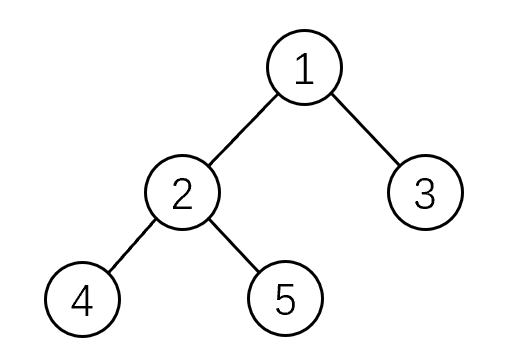
\includegraphics[width=0.25\textwidth]{assets/pics_and_ppts/ch4/习题_寻找公共祖先答案图.png}
\end{center}

第一步，当前节点root是 1，它既不是 4，也不是 5。
因此，算法继续向下查找：\\
- 左子树：从节点 2 开始。\\
- 右子树：从节点 3 开始。\\

第二步：进入节点 2，
节点 2 又会向左右子树查找：\\
- 左边进入节点 4。\\
- 右边进入节点 5。

当递归来到节点 4 时，发现它就是目标节点，于是直接返回节点 4。
同理，来到节点 5 时，直接返回节点 5。
于是，节点 2 这一层得到：
\begin{center}
    node* left = LowestCommonAncestor(root->lchild, 4, 5);       // left是节点4的指针 \\
    node* right = LowestCommonAncestor(root->rchild, 4, 5);     // right是节点5的指针
\end{center}
两边都不为空！说明两个目标节点分别出现在节点 2 的左右子树中。
因此，返回节点 2。\\

第三步：返回节点 1，
节点 2的递归函数中 返回了节点 2，意味着节点 1 的左侧查找结果是节点 2。
而节点 3 的子树里没有 4 或 5，所以右侧返回 nullptr。
因此，节点 1 得到：
\begin{center}
    node* left = LowestCommonAncestor(root->lchild, 4, 5);       // left是节点2的指针 \\
    node* right = LowestCommonAncestor(root->rchild, 4, 5);     // right是NULL
\end{center}
因为只有左边有结果，节点 1的递归函数栈中 就把左边的结果（节点2的指针）继续返回。
得到最终答案是节点 2。\\

8. 事实上有两点可以优化：\\
1）若a和b与某节点相比一大一小，则该节点一定就是最近公共祖先，而无需继续向下找a和b；\\
2）a和b都更大或都更小时，无需两棵子树都进行递归，拿到left和right的信息，而是直接进入lchild或rchild即可。 

此外，由于查找结点一定存在，而在二叉查找树下由上面的2），我们能确定每次递归进入的路径下方一定存在公共祖先，因此一定不会进入NULL节点。
\begin{cppcode}
    node* LowestCommonAncestor(node* root, int a, int b) {
        // a和b分别在root的左右子树中，root就是最近公共祖先
        if(a < root->key && b > root->key) return root;
        if(a > root->key && b < root->key) return root;

        // root就是a或b，root一定是最近公共祖先
        if(root->key == a || root->key == b) return root;
        // a和b都在左子树或都在右子树中，递归地进入左子树或右子树。
        if(a > root->key && b > root->key) return LowestCommonAncestor(root->right, a, b);
        return LowestCommonAncestor(root->left, a, b);
    }
\end{cppcode}

\vspace{\baselineskip}

9. 中序遍历中，第k个访问的节点就是树中第k小的元素。因此我们可以在中序遍历过程中，用一个变量visited\_num记录当前已经有多少个节点被访问过了。
当访问到某节点使得 visited\_num == k 时，返回该节点即可，代码如下。

\begin{cppcode}
    void InOrderTravel(node* root, int k, int& visited_num, int& result) {
        if(root == NULL) return ;
        InOrderTravel(root->lchild, k, visited_num, result);

        // 代码执行到此处时，才是中序遍历中“访问”一个节点的时候
        visited_num += 1;
        if(visited_num == k) {
            result = root->val;
            return ;
        }
        // 若visited_num已经>=k，说明找到了，无需继续递归遍历了。
        if(visited_num < k) {
            InOrderTravel(root->rchild, k, visited_num, result);
        }
    }
    int kthSmallest(node* root, int k) {
        int result = 0;
        int visited_num = 0;
        InOrderTravel(root, k, visited_num, result);
        return result;
    }
\end{cppcode}

\vspace{\baselineskip}

10. 相信一定有人的思路是这样：遍历一遍所有节点i，判断：其左孩子（即2i）小于节点i的值，并且其右孩子（即2i+1）大于节点i的值，若存在一个节点该条件不成立，则返回false。
否则返回true。事实上，这种思路是错误的。如图，
\begin{center}
    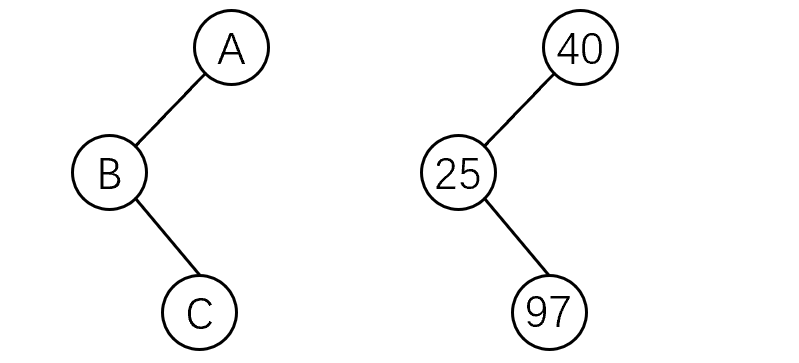
\includegraphics[width=0.35\textwidth]{assets/pics_and_ppts/ch4/22408错误思路示例.png}
\end{center}
以上思路能保证B<A、B<C成立，但不能保证C<A成立。正确的做法是：\\

【解法一】遍历一遍所有节点，不能只判断其左右孩子，而是要判断其左子树中的最大值是否满足小于该节点的值、右子树中的最小值是否满足大于该节点的值。只有所有
节点都满足以上条件，才是一棵二叉搜索树。

我们维护两个数组：local\_min[]和local\_max[]，local\_min[i] 和 local\_max[i] 的值分别表示以节点i为根的子树中的最小值和最大值。从后向前遍历一遍所有节点，
判断是否满足二叉搜索树条件的同时，更新这两个数组。具体过程请参见代码及注释。

\begin{cppcode}
    bool IsBST(SqBiTree tree) {
        // local_max[i]、local_min[i]分别表示以i为根的子树中元素的最大、最小值
        int local_max[MAX_SIZE];
        int local_min[MAX_SIZE];
        // 每个节点为根的子树，其中最大或最小值至少是它们自己
        for(int i=0; i<MAX_SIZE; ++i) {
            local_min[i] = local_max[i] = tree.SqBiTNode[i];
        }

        for(int i=tree.ElemNum; i>=1; i--) {
            int lchild_idx = 2*i;
            int rchild_idx = 2*i+1;

            // 节点i有左孩子
            if(lchild_idx <= tree.ElemNum && tree.SqBiTNode[lchild_idx] != -1) {  
                if(tree.SqBiTNode[i] <= local_max[lchild_idx]) {    // 当前节点的值小于等于左子树中的最大值，不符合条件，返回false
                    return false;
                }
                // 以该节点i为根的子树中的最小值更新为i的左子树中的最小值。
                local_min[i] = local_min[lchild_idx];
            }

            // 节点i有右孩子
            if(rchild_idx <= tree.ElemNum && tree.SqBiTNode[rchild_idx] != -1) {    
                if(tree.SqBiTNode[i] >= local_min[rchild_idx]) {    // 当前节点的值大于等于右子树中的最小值，不符合条件，返回false
                    return false;
                }
                // 以该节点i为根的子树中的最大值更新为i的右子树中的最大值。
                local_max[i] = local_max[rchild_idx];
            }
        } // end for()
        
        // 以上for循环结束，说明所有节点均满足二叉搜索树的条件，返回true。
        return true;
    }
\end{cppcode}


\vspace{\baselineskip}

【解法二】本题还有一种更简单的解法：根据二叉搜索树中序遍历一定是有序的，我们在中序遍历的过程中，记录当前访问的节点i的中序前驱的值pre，若存在某个节点，
其值小于等于pre，则返回false。

\begin{cppcode}
    void InOrderTravel(SqBiTree tree, int i, int& pre, bool& ans);

    bool IsBST(SqBiTree tree) {
        // 先假设是二叉搜索树，若遍历过程发现不满足，将ans置为false。
        bool ans = true;
        // 树中节点都是正整数，因此将第一个节点的前驱初始化为0或任意负数即可。
        int pre = -10;
        InOrderTravel(tree, 1, pre, ans);
        return ans;
    }

    void InOrderTravel(SqBiTree tree, int i, int& pre, bool& ans) {
        // 节点不存在，直接返回
        if(i > tree.ElemNum || tree.SqBiTNode[i] == -1) return;
        // 已经可以做否定断定，无需继续遍历
        if(ans == false) return ;

        // 先访问左子树
        InOrderTravel(tree, 2*i, pre, ans);

        // 若当前访问节点小于等于其前驱，说明不是二叉搜索树
        if(tree.SqBiTNode[i] <= pre) {
            ans = false;
            return;
        }
        // 将下一个待访问节点的中序前驱更新为当前节点
        pre = tree.SqBiTNode[i];

        // 访问右子树
        InOrderTravel(tree, 2*i+1, pre, ans);
        return;
    }
\end{cppcode}




\end{exerciseanswer}%%%%%%%%%%%%%%%%%%%%%%%%%%%%%%%%%%%%%%%%%%%%%%%%%%%%%%%%%%%%%%%%%%%%%%%%%%%%%%%%%%%%%%%%%%%%%%%%%%%%%%%%%%%%%%%%%%%%%%%%%%%%%%%%%%%%


